\section{Mức 9,10 điểm}
\setcounter{ex}{0}
\setcounter{dang}{0}
\Opensolutionfile{ans}[ans/CD1/Muc_9_10]
\begin{dang}{Tìm m để hàm số đơn điệu trên các khoảng xác định của nó}
	Đang thiếu bài thầy Jf Câu 1 đến 26 
\end{dang}
\begin{dang}
	{Tìm khoảng đơn điệu của hàm số $g(x) = f\left[ u(x)\right] +v(x)$ khi biết đồ thị hoặc bảng biến thiên của hàm số $y = f'(x)$}
\end{dang}
\begin{ex}[Đề tham khảo 2019]%[2D1K1-2]
	Cho hàm số $f(x)$ có bảng xét dấu của đạo hàm như sau
	\begin{center}
		
\begin{tikzpicture}
			\tkzTabInit[nocadre,lgt=1.2,espcl=2,deltacl=0.6]
			{$x$ /0.6,$f'(x)$ /0.6}
			{$-\infty$,$1$,$2$,$3$,$4$,$+\infty$}
			\tkzTabLine{,-,$0$,+,$0$,+,$0$,-,$0$,+,}
		\end{tikzpicture}
	\end{center}
	Hàm số $y=3 f(x+2)-x^3+3 x$ đồng biến trên khoảng nào dưới đây?
	\choice
	{$(-\infty ;-1)$}
	{\True $(-1 ; 0)$}
	{$(0 ; 2)$}
	{$(1 ;+\infty)$}
	\loigiai{
		Ta có $y'=3\left[f'(x+2)-\left(x^2-3\right)\right]$.\\
		Với $x \in(-1 ; 0) \Rightarrow x+2 \in(1 ; 2) \Rightarrow f'(x+2)>0$, lại có $x^2-3<0 \Rightarrow y'>0 ;~ \forall x \in(-1 ; 0)$.\\
		Vậy hàm số $y=3 f(x+2)-x^3+3 x$ đồng biến trên khoảng $(-1 ; 0)$.\\
		Chú ý:\\
		+) Ta xét $x \in(1 ; 2) \subset(1 ;+\infty)
		\Rightarrow x+2 \in(3 ; 4)\\
		\Rightarrow f'(x+2)<0 ;~ x^2-3>0$\\
		Suy ra hàm số nghịch biến trên khoảng $(1 ; 2)$ nên loại hai phương án$(0 ; 2)$ và $(1 ;+\infty)$.\\
		+) Tương tự ta xét
		$x \in(-\infty ;-2) \Rightarrow x+2 \in(-\infty ; 0)\\
		\Rightarrow f'(x+2)<0 ; x^2-3>0 \Rightarrow y'<0 ; ~ \forall x \in(-\infty ;-2)$.\\
		Suy ra hàm số nghịch biến trên khoảng $(-\infty ;-2)$ nên loại$(-\infty ;-1)$.\\
		Vậy hàm số đã cho đồng biến trên khoảng $(-1 ; 0)$.
	}
\end{ex}
\begin{ex}[Đề Tham Khảo 2020 - Lần 1]%[2D1G1-2]
	\immini{
		Cho hàm số $f(x)$. Hàm số $y=f'(x)$ có đồ thị như hình bên. Hàm số $g(x)=f(1-2 x)+x^2-x$ nghịch biến trên khoảng nào dưới đây?
		\choice
		{\True $\left(1 ; \dfrac{3}{2}\right)$}
		{$\left(0 ; \dfrac{1}{2}\right)$}
		{$(-2 ;-1)$}
		{$(2 ; 3)$}
	}
	{
		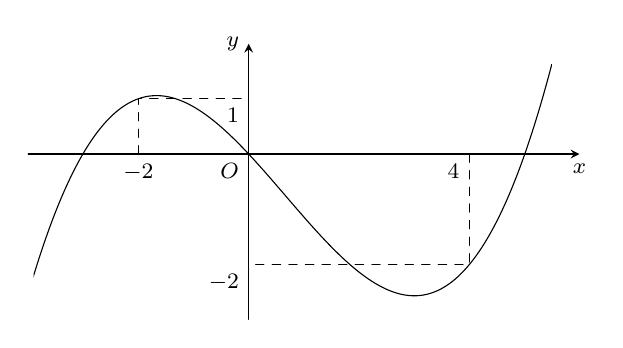
\begin{tikzpicture}[scale=0.7,>=stealth, font=\footnotesize, line join=round, line cap=round]
			%\def\a{1} \def\b{-6} \def\c{9} \def\d{1} % Hệ số
			\def\xmin{-4} \def\xmax{6}
			\def\ymin{-3} \def\ymax{2} 
			%\draw[color=gray!50,dashed] (\xmin,\ymin) grid (\xmax,\ymax); 
			\draw[->] (\xmin,0)--(\xmax,0) node [below]{$x$};
			\draw[->] (0,\ymin)--(0,\ymax) node [left]{$y$};
			\node at (0,0) [below left]{$O$};
			%\node at (1,3) [below left]{$f'(x)$};
			%\node at (-1.3,4) {$f'(x)$};
			\draw[dashed] (-2,0) node[below]{$-2$}--(-2,1)--(0,1) node[below left]{$1$};
			\draw[dashed] (4,0) node[below left]{$4$}--(4,-2)--(0,-2) node[below left]{$-2$};
			%\draw[dashed] (1,0) node[below]{$1$}--(1,1);
			%\draw[dashed] (-0.5,0) node[below left]{$-0{,}5$}--(-0.5,2.125);
			\clip (\xmin+0.1,\ymin+0.1) rectangle (\xmax-0.5,\ymax-0.1);
			\draw[smooth,samples=300][domain=-4:5.5] plot(\x,{0.071*(\x)^3-0.142*(\x)^2-1.07*(\x)});
		\end{tikzpicture}
	}
	
	\loigiai{
		Ta có : $g(x)=f(1-2 x)+x^2-x \Rightarrow g'(x)=-2 f'(1-2 x)+2 x-1$.\\
		\immini{
			Đặt $t=1-2 x \Rightarrow g'(x)=-2 f'(t)-t$.\\
			$g'(x)=0 \Rightarrow f'(t)=-\dfrac{t}{2}$.\\
			Vẽ đường thẳng $y=-\dfrac{x}{2}$ và đồ thị hàm số $f'(x)$ trên cùng một hệ trục
		}	
		{
			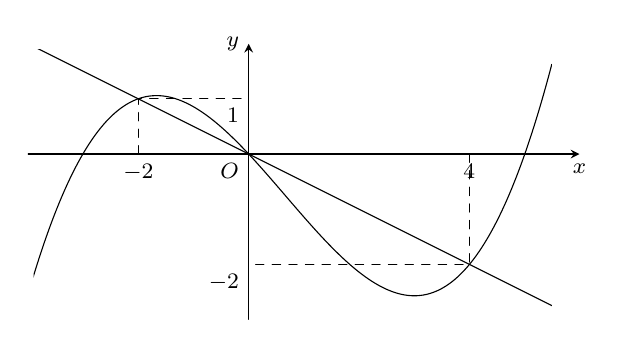
\begin{tikzpicture}[scale=0.7,>=stealth, font=\footnotesize, line join=round, line cap=round]
				%\def\a{1} \def\b{-6} \def\c{9} \def\d{1} % Hệ số
				\def\xmin{-4} \def\xmax{6}
				\def\ymin{-3} \def\ymax{2} 
				%	\draw[color=gray!50,dashed] (\xmin,\ymin) grid (\xmax,\ymax); 
				\draw[->] (\xmin,0)--(\xmax,0) node [below]{$x$};
				\draw[->] (0,\ymin)--(0,\ymax) node [left]{$y$};
				\node at (0,0) [below left]{$O$};
				%\node at (1,3) [below left]{$f'(x)$};
				%\node at (-1.3,4) {$f'(x)$};
				\draw[dashed] (-2,0) node[below]{$-2$}--(-2,1)--(0,1) node[below left]{$1$};
				\draw[dashed] (4,0) node[below]{$4$}--(4,-2)--(0,-2) node[below left]{$-2$};
				%\draw[dashed] (1,0) node[below]{$1$}--(1,1);
				%\draw[dashed] (-0.5,0) node[below left]{$-0{,}5$}--(-0.5,2.125);
				\clip (\xmin+0.1,\ymin+0.1) rectangle (\xmax-0.5,\ymax-0.1);
				\draw[smooth,samples=300][domain=-4:5.5] plot(\x,{0.071*(\x)^3-0.142*(\x)^2-1.07*(\x)});
				\draw[smooth,samples=300][domain=-4:5.5] plot(\x,{(-0.5*(\x)});
			\end{tikzpicture}
		}	Hàm số $g(x)$ nghịch biến $\Rightarrow g'(x) \leq 0 \Rightarrow f'(t) \geq-\dfrac{t}{2}\Rightarrow\hoac{&-2 \leq t \leq 0 \\&t \geq 4.}$\\
		Như vậy $f'(1-2 x) \geq \dfrac{1-2 x}{-2}\Rightarrow\hoac{&-2 \leq 1-2 x \leq 0 \\ &4 \leq 1-2 x}\Rightarrow\hoac{&\dfrac{1}{2}\leq x \leq \dfrac{3}{2}\\ &x \leq-\dfrac{3}{2}.}$\\
		Vậy hàm số $g(x)=f(1-2 x)+x^2-x$ nghịch biến trên các khoảng $\left(\dfrac{1}{2}; \dfrac{3}{2}\right)$ và $\left(-\infty ;-\dfrac{3}{2}\right)$.\\
		Mà $\left(1 ; \dfrac{3}{2}\right) \subset \left(\dfrac{1}{2}; \dfrac{3}{2}\right)$ nên hàm số $g(x)=f(1-2 x)+x^2-x$ nghịch biến trên khoảng $\left(1 ; \dfrac{3}{2}\right)$.
	}
\end{ex}
\begin{ex}[Chuyên Lê Quý Đôn Điện Biên 2019]%[2D1G1-2]
	Cho hàm số $f(x)$ có bảng xét dấu của đạo hàm như sau
	\begin{center}
		
\begin{tikzpicture}
			\tkzTabInit[nocadre,lgt=1.2,espcl=2,deltacl=0.6]
			{$x$ /0.6,$f'(x)$ /0.6}
			{$-\infty$,$0$,$1$,$2$,$3$,$+\infty$}
			\tkzTabLine{,+,$0$,-,$0$,-,$0$,+,$0$,-,}
		\end{tikzpicture}
	\end{center}
	Hàm số $y=f(x-1)+x^3-12 x+2019$ nghịch biến trên khoảng nào dưới đây?
	\choice
	{$(1 ;+\infty)$}
	{\True $(1 ; 2)$}
	{$(-\infty ; 1)$}
	{$(3 ; 4)$}
	\loigiai{
		$y'=f'(x-1)+3 x^2-12=f'(t)+3 t^2+6 t-9=f'(t)-\left(-3 t^2-6 t+9\right)$, với $t=x-1$.\\
		\immini{
			Nghiệm của phương trình $y'=0$ là hoành độ giao điểm của các đồ thị hàm số $y=f'(t)$ và $y=-3 t^2-6 t+9$.\\
			Vẽ đồ thị hàm số $y=f'(t)$ và $y=-3 t^2-6 t+9$ trên cùng một hệ trục tọa độ như hình vẽ bên.
		}	
		{		\begin{tikzpicture}[scale=0.5,>=stealth, font=\footnotesize, line join=round, line cap=round]
				\def\a{-3} \def\b{-6} \def\c{9} % Hệ số
				\def\xmin{-9} \def\xmax{7}
				\def\ymin{-3} \def\ymax{13}
				
				%\draw[color=gray!50,dashed] (\xmin,\ymin) grid (\xmax,\ymax);
				
				\draw[->] (\xmin,0)--(\xmax,0) node [below]{$x$};
				\draw[->] (0,\ymin)--(0,\ymax) node [left]{$y$};
				\node at (0,0) [below left]{$O$};
				\clip (\xmin+0.1,\ymin+0.1) rectangle (\xmax-0.5,\ymax-0.1);
				\draw[smooth,samples=300] plot(\x,{\a*(\x)^2+\b*(\x)+\c});
				\node at (1,0) [above right]{$1$};
				\node at (2,0) [below right]{$2$};
				\node at (3,0) [below right]{$3$};
				\node at (-3,-2) [left]{$y=-3t^2-6t+9$};
				\node at (4,0) [below right]{$f'(x)$};
				\draw (-2.2,10).. controls (-1,1.9) and (-0.5,0.8) .. (0,0);
				%\draw (-2,0).. controls (-1.5,-2) and (-0.5,-0) .. (0,0);
				\draw (0,0).. controls (0.4,-0.6) and (0.6,-0.6) .. (0.8,-0.2);
				\draw (0.8,-0.2).. controls (1,0.25) and (1.1,-0.1) .. (1.4,-0.8);
				\draw (1.4,-0.8).. controls (1.6,-1.1) and (1.7,-0.9) .. (2,0);
				\draw (2,0).. controls (2.4,1.1) and (2.6,1.1) .. (3.5,-1);
			\end{tikzpicture}
		}
		Dựa vào đồ thị trên, ta có bảng xét dấu của hàm số $y'=f'(t)-\left(-3 t^2-6 t+9\right)$ như sau $
		\left(t_0<-1\right)$
		\begin{center}
			
\begin{tikzpicture}
				\tkzTabInit[nocadre,lgt=2,espcl=2,deltacl=0.6]
				{$x$ /0.6,$y'$ /0.6}
				{$-\infty$,$t_0$,$1$,$+\infty$}
				\tkzTabLine{,+,$0$,-,$0$,+,}
			\end{tikzpicture}
		\end{center}
		Hàm số nghịch biến trên khoảng $t \in\left(t_0 ; 1\right)$.\\
		Do đó hàm số nghịch biến trên khoảng $x \in(1 ; 2) \subset \left(t_0+1 ; 1\right)$.
	}
\end{ex}


\begin{ex}[Chuyên Phan Bội Châu Nghệ An 2019]%[2D1G1-2]
	Cho hàm số $f(x)$ có bảng xét dấu đạo hàm như sau:
	\begin{center}
		
\begin{tikzpicture}
			\tkzTabInit[nocadre,lgt=2,espcl=2,deltacl=0.6]
			{$x$ /0.6,$f'(x)$ /0.6}
			{$-\infty$,$1$,$2$,$3$,$4$,$+\infty$}
			\tkzTabLine{,-,$0$,+,$0$,+,$0$,-,$0$,+,}
		\end{tikzpicture}
	\end{center}
	Hàm số $y=2 f(1-x)+\sqrt{x^2+1}-x$ nghịch biến trên những khoảng nào dưới đây
	\choice
	{$(-\infty ;-2)$}
	{$(-\infty ; 1)$}
	{\True $(-2 ; 0)$}
	{$(-3 ;-2)$}
	\loigiai{
		$y'=-2 f'(1-x)+\dfrac{x}{\sqrt{x^2+1}}-1$. \\
		Có $\dfrac{x}{\sqrt{x^2+1}}-1<0,~ \forall x \in(-2 ; 0)$.\\
		Bảng xét dấu:
		\begin{center}
			
\begin{tikzpicture}
				\tkzTabInit[nocadre,lgt=2,espcl=2,deltacl=0.6]
				{$x$ /0.7,$f'(1-x)$ /0.7}
				{$-\infty$,$-3$,$-2$,$-1$,$0$,$+\infty$}
				\tkzTabLine{,+,$0$,-,$0$,+,$0$,+,$0$,-,}
			\end{tikzpicture}
		\end{center}
		$\Rightarrow-2 f'(1-x)<0, ~ \forall x \in(-2 ; 0) \\
		\Rightarrow-2 f'(1-x)+\dfrac{x}{\sqrt{x^2+1}}-1<0, ~\forall x \in(-2 ; 0)$.
	}
\end{ex}
\begin{ex}[Sở Vĩnh Phúc 2019]%[2D1G1-2]
	\immini{
		Cho hàm số bậc bốn $y=f(x)$ có đồ thị của hàm số $y=f'(x)$ như hình vẽ bên.\\
		Hàm số $y=3 f(x)+x^3-6 x^2+9 x$ đồng biến trên khoảng nào trong các khoảng sau đây?
		\choice
		{$(0 ; 2)$}
		{$(-1 ; 1)$}
		{$(1 ;+\infty)$}
		{\True $(-2 ; 0)$}
	}
	{
		\begin{tikzpicture}[scale=0.7,>=stealth, font=\footnotesize, line join=round, line cap=round]
			\def\a{0.21} \def\b{0.88} \def\c{-0.58} \def\d{-3} % Hệ số
			\def\xmin{-5} \def\xmax{5}
			\def\ymin{-4} \def\ymax{3} 
			%\draw[color=gray!50,dashed] (\xmin,\ymin) grid (\xmax,\ymax); 
			\draw[->] (\xmin,0)--(\xmax,0) node [below]{$x$};
			\draw[->] (0,\ymin)--(0,\ymax) node [left]{$y$};
			\node at (0,0) [above left]{$O$};
			\node at (-4,0) [below left]{$-4$};
			\node at (-2,0) [below left]{$-2$};
			\node at (0,-3) [below right]{$-3$};
			\draw[dashed] (2,0) node[above right]{$2$}--(2,1) --(0,1) node[above right]{$1$};
			\clip (\xmin+0.1,\ymin+0.1) rectangle (\xmax-0.5,\ymax-0.1);
			\draw[smooth,samples=300] plot(\x,{\a*(\x)^3+\b*(\x)^2+\c*(\x)+\d});
		\end{tikzpicture}
	}
	
	\loigiai{
		Hàm số $f(x)=a x^4+b x^3+c x^2+d x+e,(a \neq 0)$.
		Có $f'(x)=4 a x^3+3 b x^2+2 c x+d$.\\
		Đồ thị hàm số $y=f'(x)$ đi qua các điểm $(-4 ; 0),(-2 ; 0),(0 ;-3),(2 ; 1)$ nên ta có
		$$\heva{&- 2 5 6 a + 4 8 b - 8 c + d = 0\\
			&- 3 2 a + 1 2 b - 4 c + d = 0\\
			&d = - 3\\
			&3 2 a + 1 2 b + 4 c + d = 1}\Leftrightarrow \heva{&
			a=\dfrac{5}{96}\\
			&b=\dfrac{7}{24}\\
			&c=-\dfrac{7}{24}\\
			&d=-3.}
		$$
		Xét hàm số
		$
		y=3 f(x)+x^3-6 x^2+9 x$\\
		Ta có $ y'=3\left(f'(x)+x^2-4 x+3\right)=3\left(\frac{5}{24}x^3+\frac{15}{8}x^2-\frac{55}{12}x\right)
		$\\
		Ta có $y'=0 \Leftrightarrow\hoac{&x=-11 \\&x=0 \\&x=2.}$ \\
		Xét dấu $y'$, ta được hàm số đã cho đồng biến trên các khoảng $(-11 ; 0)$ và $(2 ;+\infty)$.
	}
\end{ex}
\begin{ex}[Học Mãi 2019]%[2D1K1-2]
	\immini
	{Cho hàm số $y=f(x)$ có đạo hàm trên $\mathbb{R}$. Đồ thị hàm số $y=f'(x)$ như hình bên. Hỏi đồ thị hàm số $y=f(x)-2 x$ có bao nhiêu điểm cực trị?
		\choice
		{$4$}
		{\True $3$}
		{$2$}
		{$1$}
	}
	{
		\begin{tikzpicture}[font=\footnotesize,line join=round, line cap=round,>=stealth,scale=0.8]
			\draw[->] (-3.5,0)--(4,0) node[above] {$x$};
			\draw[->] (0,-3)--(0,4) node[left] {$y$};
			%\fill[black] (-2,0)node[below left]{$-2$} circle (1.2pt) (0,0)node[above right]{$O$} circle (1.2pt) (3,0)node[above]{$3$} circle (1.2pt);
			\draw[dashed] (-2,-2)-- (0,-2) node[right]{$-2$};
			\draw[dashed] (2,0) node[below]{$2$}-- (2,2)--(0,2) node[below left]{$2$};
			\node at (0,0) [below left]{$O$};
			\node at (3,0) [below right]{$3$};
			\draw (-3,2.5).. controls (-2.2,-3) and (-1.8,-3) .. (-1.1,0);
			\draw (-1.1,0).. controls (-0.6,2.5) and (-0.4,2.5) .. (0,2);
			\draw (0,2).. controls (0.7,0.5) and (1.1,0.5) .. (1.5,1.5);
			\draw (1.5,1.5).. controls (2,2.5) and (2.8,2.5) .. (3.5,-2.5);
			%\draw (3,0).. controls (3.3,-0.1) and (3.5,-0.5) .. (3.5,-2);
		\end{tikzpicture}
	}
	\loigiai{
		\immini{
			Đặt $g(x)=f(x)-2 x$.\\
			$\Rightarrow g'(x)=f'(x)-2 .
			$\\
			Vẽ đường thẳng $y=2$.\\
			$\Rightarrow$ phương trình $g'(x)=0$ có $3$ nghiệm bội lẻ.\\
			$\Rightarrow$ đồ thị hàm số $y=f(x)-2 x$ có $3$ điểm cực trị.
		}
		{
			\begin{tikzpicture}[font=\footnotesize,line join=round, line cap=round,>=stealth,scale=0.8]
				\draw[->] (-3.5,0)--(4,0) node[above] {$x$};
				\draw[->] (0,-3)--(0,4) node[left] {$y$};
				%\fill[black] (-2,0)node[below left]{$-2$} circle (1.2pt) (0,0)node[above right]{$O$} circle (1.2pt) (3,0)node[above]{$3$} circle (1.2pt);
				\draw[dashed] (-2,-2)-- (0,-2) node[right]{$-2$};
				\draw[dashed] (2,0) node[below]{$2$}-- (2,2)--(0,2) node[below left]{$2$};
				\node at (3,0) [below left]{$3$};
				\draw (-3,2.5).. controls (-2.2,-3) and (-1.8,-3) .. (-1.1,0);
				\draw (-1.1,0).. controls (-0.6,2.5) and (-0.4,2.5) .. (0,2);
				\draw (0,2).. controls (0.7,0.5) and (1.1,0.5) .. (1.5,1.5);
				\draw (1.5,1.5).. controls (2,2.5) and (2.8,2.5) .. (3.5,-2.5);
				\draw (-3.5,2)--(4,2) node[above]{$y=2$};
			\end{tikzpicture}
		}
	}
\end{ex}
\begin{ex}[THPT Hoàng Hoa Thám Hưng Yên 2019]%[2D1G1-2]
	\immini{
		Cho hàm số $y=f(x)$ liên tục trên $\mathbb{R}$. Hàm số $y=f'(x)$ có đồ thị như hình vẽ. 
		Hàm số $g(x)=f(x-1)+\dfrac{2019-2018 x}{2018}$ đồng biến trên khoảng nào dưới đây?
		\choice
		{$(2 ; 3)$}
		{$(0 ; 1)$}
		{\True $(-1 ; 0)$}
		{$(1 ; 2)$}
	}
	{
		\begin{tikzpicture}[scale=1, font=\footnotesize, line join=round, line cap=round, >=stealth]
			\tikzset{label style/.style={font=\footnotesize}}
			\draw[->] (-2,0)--(3,0) node[below left] {$x$};
			\draw[->] (0,-2)--(0,3) node[below left] {$y$};
			\draw[fill=black] (0,0) node [above left] {$O$} circle(1pt);
			\fill (1,1) circle(1pt) (-1,1) circle(1pt) (2,1) circle(1pt);
			\foreach \x in {1,2}
			\draw[thin] (\x,1pt)--(\x,-1pt) node [below] {\footnotesize$\x$};
			\foreach \x in {-1}
			\draw[thin] (\x,1pt)--(\x,-1pt) node [below left] {\footnotesize$\x$};
			\foreach \y in {-1}
			\draw[thin] (1pt,\y)--(-1pt,\y) node [right] {\footnotesize$\y$};
			\foreach \y in {1}
			\draw[thin] (1pt,\y)--(-1pt,\y) node [above left] {\footnotesize$\y$};
			\draw[dashed](-1,0)--(-1,1)--(2,1) (1,1)--(1,0) (2,1)--(2,0);
			\begin{scope}
				\clip (-3,-3) rectangle (3,3);
				\draw[name path=(C)] plot[smooth,tension=0.7] coordinates{(-1.15,3)(-0.5,-1.6)(.8,.88)(1.9,0.8)(2.3,3)};
			\end{scope}
		\end{tikzpicture}
	}	\loigiai{
		Ta có $g'(x)=f'(x-1)-1$.\\
		$
		g'(x) \geq 0 \Leftrightarrow f'(x-1)-1 \geq 0 \Leftrightarrow f'(x-1) \geq 1 \Leftrightarrow \hoac{&x - 1 \leq - 1\\
			&x - 1 \geq 2}\Leftrightarrow \hoac{&
			x \leq 0 \\
			&x \geq 3.}
		$\\
		Từ đó suy ra hàm số $g(x)=f(x-1)+\dfrac{2019-2018 x}{2018}$ đồng biến trên khoảng $(-1 ; 0)$.
	}
\end{ex}

\begin{ex}[(Sở Ninh Bình 2019]%[2D1K1-2]
	Cho hàm số $y=f(x)$ có bảng xét dấu của đạo hàm như sau
	\begin{center}
		
\begin{tikzpicture}
			\tkzTabInit[nocadre,lgt=1,espcl=2,deltacl=0.6]
			{$x$ /0.7,$f'(x)$ /0.7}
			{$-\infty$,$-2$,$-1$,$2$,$4$,$+\infty$}
			\tkzTabLine{,+,$0$,-,$0$,+,$0$,-,$0$,+,}
		\end{tikzpicture}
	\end{center}
	Hàm số $y=-2 f(x)+2019$ nghịch biến trên khoảng nào trong các khoảng dưới đây?
	\choice
	{$(-4 ; 2)$}
	{\True $(-1 ; 2)$}
	{$(-2 ;-1)$}
	{$(2 ; 4)$}
	\loigiai{
		Xét $y=g(x)=-2 f(x)+2019$.\\
		Ta có $g'(x)=(-2 f(x)+2019)'=-2 f'(x), g'(x)=0 \Leftrightarrow\hoac{&x=-2 \\&x=-1 \\&x=2 \\&x=4.}$.\\
		Ta có bảng xét dấu của $g'(x)$
		\begin{center}
			
\begin{tikzpicture}
				\tkzTabInit[nocadre,lgt=1,espcl=2,deltacl=0.6]
				{$x$ /0.6,$f'(x)$ /0.6}
				{$-\infty$,$-2$,$-1$,$2$,$4$,$+\infty$}
				\tkzTabLine{,-,$0$,+,$0$,-,$0$,+,$0$,+,}
			\end{tikzpicture}
		\end{center}
		Dựa vào bảng xét dấu, ta thấy hàm số $y=g(x)$ nghịch biến trên khoảng $(-1 ; 2)$.
	}
\end{ex}
\begin{ex}[THPT Lương Thế Vinh Hà Nội 2019]%[2D1G1-2]
	\immini{
		Cho hàm số $y=f(x)$. Biết đồ thị hàm số $y=f'(x)$ có đồ thị như hình vẽ bên. 
		Hàm số $y=f \left(3-x^2\right)+2018$ đồng biến trên khoảng nào dưới đây?
		\choice
		{\True $(-1 ; 0)$}
		{$(2 ; 3)$}
		{$(-2 ;-1)$}
		{$(0 ; 1)$}
	}
	{
		\begin{tikzpicture}[scale=0.6,>=stealth, font=\footnotesize, line join=round, line cap=round]
			\def\a{0.065} \def\b{0.32} \def\c{-0.53} \def\d{-0.82} % Hệ số
			\def\xmin{-8} \def\xmax{4}
			\def\ymin{-3} \def\ymax{3} 
			%\draw[color=gray!50,dashed] (\xmin,\ymin) grid (\xmax,\ymax); 
			\draw[->] (\xmin,0)--(\xmax,0) node [below]{$x$};
			\draw[->] (0,\ymin)--(0,\ymax) node [left]{$y$};
			\node at (0,0) [below left]{$O$};
			\node at (-6,0) [below left]{$-6$};
			\node at (-1,0) [below left]{$-1$};
			\node at (2,0) [below right]{$2$};
			\clip (\xmin+0.1,\ymin+0.1) rectangle (\xmax-0.5,\ymax-0.1);
			\draw[smooth,samples=300][domain=-6.5:3.5] plot(\x,{\a*(\x)^3+\b*(\x)^2+\c*(\x)+\d});
		\end{tikzpicture}
	}
	
	\loigiai{
		Ta có $\left[f\left( 3-x^2\right)+2018 \right]'=-2 x \cdot f'\left(3-x^2\right) $.\\
		$
		-2 x \cdot f'\left(3-x^2\right)=0 \Leftrightarrow\hoac{&
			x = 0\\
			&3 - x ^{2}= - 6\\
			&3 - x ^{2}= - 1\\
			&3 - x ^{2}= 2}
		\Leftrightarrow \hoac{
			&x=0 \\
			&x=\pm 3 \\
			&x=\pm 2 \\
			&	x=\pm 1.}
		$\\
		Bảng xét dấu của đạo hàm hàm số đã cho
		\begin{center}
			\begin{center}
				
\begin{tikzpicture}
					\tkzTabInit[nocadre,lgt=2.9,espcl=1.5,deltacl=0.6]
					{$x$ /0.7,$f'\left( 3-x^2\right) $/0.7,$-2xf'\left( 3-x^2\right)$/0.8}
					{$-\infty$,$-3$,$-2$,$-1$,$0$,$1$,$2$,$3$,$+\infty$}
					\tkzTabLine{,-,$0$,+,$0$,-,$0$,+,$0$,+,$0$,-,$0$,+,$0$,-}
					\tkzTabLine{,-,$0$,+,$0$,-,$0$,+,$0$,-,$0$,+,$0$,-,$0$,+}
				\end{tikzpicture}
			\end{center}
		\end{center}
		Từ bảng xét dấu suy ra hàm số đồng biến trên $(-1 ; 0)$.
	}
\end{ex}
\begin{ex}[Chuyên Biên Hòa - Hà Nam - 2020]%[2D1G1-2]
	\immini{
		Cho hàm số đa thức $f(x)$ có đạo hàm trên $\mathbb{R}$. Biết $f(0)=0$ và đồ thị hàm số $y=f'(x)$ như hình sau.
		Hàm số $g(x)=\left|4 f(x)+x^2\right|$ đồng biến trên khoảng nào dưới đây?
		\choice
		{$(4 ;+\infty)$}
		{\True $(0 ; 4)$}
		{$(-\infty ;-2)$}
		{$(-2 ; 0)$}
	}	
	{
		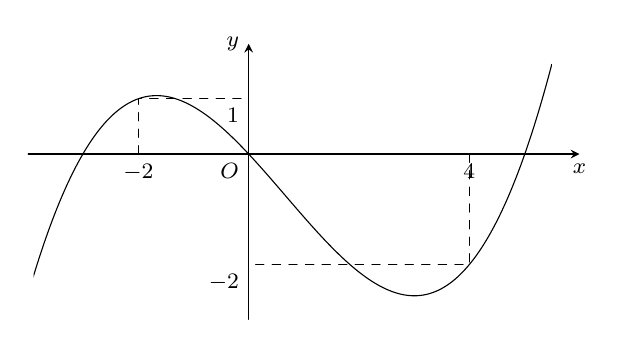
\begin{tikzpicture}[scale=0.7,>=stealth, font=\footnotesize, line join=round, line cap=round]
			%\def\a{1} \def\b{-6} \def\c{9} \def\d{1} % Hệ số
			\def\xmin{-4} \def\xmax{6}
			\def\ymin{-3} \def\ymax{2} 
			%\draw[color=gray!50,dashed] (\xmin,\ymin) grid (\xmax,\ymax); 
			\draw[->] (\xmin,0)--(\xmax,0) node [below]{$x$};
			\draw[->] (0,\ymin)--(0,\ymax) node [left]{$y$};
			\node at (0,0) [below left]{$O$};
			%\node at (1,3) [below left]{$f'(x)$};
			%\node at (-1.3,4) {$f'(x)$};
			\draw[dashed] (-2,0) node[below]{$-2$}--(-2,1)--(0,1) node[below left]{$1$};
			\draw[dashed] (4,0) node[below]{$4$}--(4,-2)--(0,-2) node[below left]{$-2$};
			%\draw[dashed] (1,0) node[below]{$1$}--(1,1);
			%\draw[dashed] (-0.5,0) node[below left]{$-0{,}5$}--(-0.5,2.125);
			\clip (\xmin+0.1,\ymin+0.1) rectangle (\xmax-0.5,\ymax-0.1);
			\draw[smooth,samples=300][domain=-4:5.5] plot(\x,{0.071*(\x)^3-0.142*(\x)^2-1.07*(\x)});
		\end{tikzpicture}
	}
	\loigiai{
		\immini{
			Xét hàm số $h(x)=4 f(x)+x^2$ trên $\mathbb{R}$.\\
			Vì $f(x)$ là hàm số đa thức nên $h(x)$ cũng là hàm số đa thức và $h(0)=4 f(0)=0$.\\
			Ta có $h'(x)=4 f'(x)+2 x$. Do đó $h'(x)=0 \Leftrightarrow f'(x)=-\dfrac{1}{2}x$.\\
		}
		{
			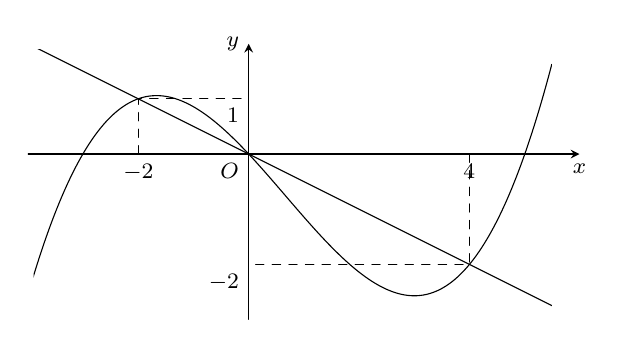
\begin{tikzpicture}[scale=0.7,>=stealth, font=\footnotesize, line join=round, line cap=round]
				%\def\a{1} \def\b{-6} \def\c{9} \def\d{1} % Hệ số
				\def\xmin{-4} \def\xmax{6}
				\def\ymin{-3} \def\ymax{2} 
				%\draw[color=gray!50,dashed] (\xmin,\ymin) grid (\xmax,\ymax); 
				\draw[->] (\xmin,0)--(\xmax,0) node [below]{$x$};
				\draw[->] (0,\ymin)--(0,\ymax) node [left]{$y$};
				\node at (0,0) [below left]{$O$};
				%\node at (1,3) [below left]{$f'(x)$};
				%\node at (-1.3,4) {$f'(x)$};
				\draw[dashed] (-2,0) node[below]{$-2$}--(-2,1)--(0,1) node[below left]{$1$};
				\draw[dashed] (4,0) node[below]{$4$}--(4,-2)--(0,-2) node[below left]{$-2$};
				%\draw[dashed] (1,0) node[below]{$1$}--(1,1);
				%\draw[dashed] (-0.5,0) node[below left]{$-0{,}5$}--(-0.5,2.125);
				\clip (\xmin+0.1,\ymin+0.1) rectangle (\xmax-0.5,\ymax-0.1);
				\draw[smooth,samples=300][domain=-4:5.5] plot(\x,{0.071*(\x)^3-0.142*(\x)^2-1.07*(\x)});
				\draw[smooth,samples=300][domain=-4:5.5] plot(\x,{-0.5*(\x)});
			\end{tikzpicture}
		}
		Dựa vào sự tương giao của đồ thị hàm số $y=f'(x)$ và đường thẳng $y=-\dfrac{1}{2}x$, ta có
		$
		h'(x)=0 \Leftrightarrow x \in\{-2 ; 0 ; 4\}.\\
		$
		Bảng biến thiên của hàm số $h(x)$ như sau:
		\begin{center}
			
\begin{tikzpicture}
				\tkzTabInit[nocadre,lgt=1.2,espcl=2.5,deltacl=0.6]
				{$x$ /0.6,$y'$ /0.6,$y$ /2}
				{$-\infty$,$-2$,$0$,$4$,$+\infty$}
				\tkzTabLine{,-,$0$,+,$0$,-,$0$,+,}
				\tkzTabVar{+/$+\infty$, -/$y_1$,+/$0$,-/$y_3$,+/$+\infty$}
			\end{tikzpicture}
		\end{center}
		Từ đó suy ra bảng biến thiên của hàm số $g(x)=|h(x)|$.\\
		Dựa vào bảng biến thiên trên, ta thấy hàm số $g(x)$ đồng biến trên khoảng $(0 ; 4)$.
	}
\end{ex}
\begin{ex}[Chuyên Thái Bình - 2020]%[2D1G1-2]
	\immini{
		Cho hàm số $f(x)$ liên tục trên $\mathbb{R}$ có đồ thị hàm số $y=f'(x)$ cho như hình vẽ bên.\\
		Hàm số $g(x)=2 f(|x-1|)-x^2+2 x+2020$ đồng biến trên khoảng nào?
		\choice
		{\True $(0 ; 1)$}
		{$(-3 ; 1)$}
		{$(1 ; 3)$}
		{$(-2 ; 0)$}
	}
	{
		\begin{tikzpicture}[scale=0.7,>=stealth, font=\footnotesize, line join=round, line cap=round]
			%\def\a{1} \def\b{-6} \def\c{9} \def\d{1} % Hệ số
			\def\xmin{-4} \def\xmax{5}
			\def\ymin{-3} \def\ymax{5} 
			%\draw[color=gray!50,dashed] (\xmin,\ymin) grid (\xmax,\ymax); 
			\draw[->] (\xmin,0)--(\xmax,0) node [below]{$x$};
			\draw[->] (0,\ymin)--(0,\ymax) node [left]{$y$};
			\node at (0,0) [below left]{$O$};
			%\node at (1,3) [below left]{$f'(x)$};
			\node at (-1.3,4) {$f'(x)$};
			\draw[dashed] (-1,0) node[above]{$-1$}--(-1,-1)--(0,-1) node[below left]{$-1$};
			\draw[dashed] (1,0) node[below]{$1$}--(1,1)--(0,1) node[below left]{$1$};
			\draw[dashed] (3,0) node[below]{$3$}--(3,3)--(0,3) node[below left]{$3$};
			%\draw[dashed] (1,0) node[below]{$1$}--(1,1);
			%\draw[dashed] (-0.5,0) node[below left]{$-0{,}5$}--(-0.5,2.125);
			\clip (\xmin+0.1,\ymin+0.1) rectangle (\xmax-0.5,\ymax-0.1);
			\draw[smooth,samples=300][domain=-2:4] plot(\x,{-0.5*(\x)^3+1.5*(\x)^2+1.5*(\x)-1.5});
			%\draw[smooth,samples=300] plot(\x,{(\x)^3+(\x)^2-2*(\x)+1});
		\end{tikzpicture}
	}
	\loigiai{
		Ta có đường thẳng $y=x$ cắt đồ thị hàm số $y=f'(x)$ tại các điểm $x=-1 ; x=1 ; x=3$ như hình vẽ sau:
		\begin{center}
			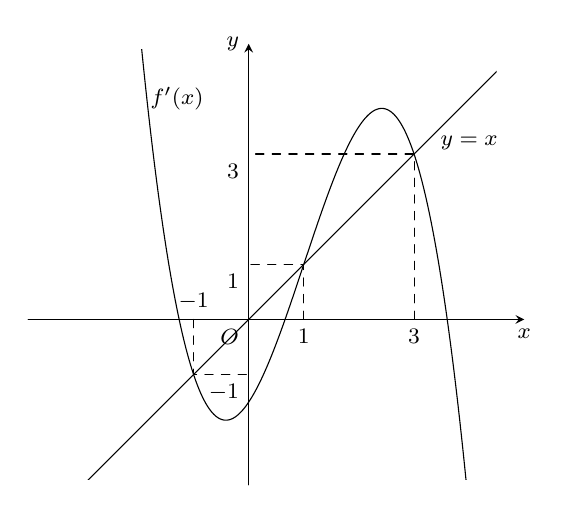
\begin{tikzpicture}[scale=0.7,>=stealth, font=\footnotesize, line join=round, line cap=round]
				%\def\a{1} \def\b{-6} \def\c{9} \def\d{1} % Hệ số
				\def\xmin{-4} \def\xmax{5}
				\def\ymin{-3} \def\ymax{5} 
				%\draw[color=gray!50,dashed] (\xmin,\ymin) grid (\xmax,\ymax); 
				\draw[->] (\xmin,0)--(\xmax,0) node [below]{$x$};
				\draw[->] (0,\ymin)--(0,\ymax) node [left]{$y$};
				\node at (0,0) [below left]{$O$};
				%\node at (1,3) [below left]{$f'(x)$};
				\node at (-1.3,4) {$f'(x)$};
				\node at (4,3.2) {$y=x$};
				\draw[dashed] (-1,0) node[above]{$-1$}--(-1,-1)--(0,-1) node[below left]{$-1$};
				\draw[dashed] (1,0) node[below]{$1$}--(1,1)--(0,1) node[below left]{$1$};
				\draw[dashed] (3,0) node[below]{$3$}--(3,3)--(0,3) node[below left]{$3$};
				%\draw[dashed] (1,0) node[below]{$1$}--(1,1);
				%\draw[dashed] (-0.5,0) node[below left]{$-0{,}5$}--(-0.5,2.125);
				\clip (\xmin+0.1,\ymin+0.1) rectangle (\xmax-0.5,\ymax-0.1);
				\draw[smooth,samples=300][domain=-2:4] plot(\x,{-0.5*(\x)^3+1.5*(\x)^2+1.5*(\x)-1.5});
				\draw[smooth,samples=300] plot(\x,{(\x)});
			\end{tikzpicture}
		\end{center}
		Dựa vào đồ thị của hai hàm số trên ta có $f'(x)>x \Leftrightarrow\hoac{&x<-1 \\ &1<x<3}$ và
		$ f'(x)<x \Leftrightarrow\hoac{&
			-1<x<1 \\
			&x>3.}$\\
		+Trường hợp 1: $x-1<0 \Leftrightarrow x<1$.\\
		Khi đó $g(x)=2 f(1-x)-x^2+2 x+2020$.\\
		Ta có $g'(x)=-2 f'(1-x)+2(1-x)$.
		$$
		g'(x)>0 \Leftrightarrow-2 f'(1-x)+2(1-x)>0 \Leftrightarrow f'(1-x)<1-x \Leftrightarrow\hoac{
			&- 1 < 1 - x < 1\\
			&1 - x > 3} \Leftrightarrow \hoac{&
			0<x<2 \\
			&x<-2.}
		$$
		Kết hợp điều kiện, ta có $g'(x)>0 \Leftrightarrow\hoac{&0<x<1 \\ &x<-2.}$\\
		
		+ Trường hợp 2: $x-1>0 \Leftrightarrow x>1$.\\
		Khi đó ta có $g(x)=2 f(x-1)-x^2+2 x+2020$.\\
		$ g'(x)=2 f'(x-1)-2(x-1)$\\
		$g'(x)>0 \Leftrightarrow 2 f'(x-1)-2(x-1)>0 \Leftrightarrow f'(x-1)>x-1 \Leftrightarrow\hoac{&
			x - 1 < - 1\\
			&1 < x - 1 < 3}\Leftrightarrow \hoac{
			&x<0 \\
			&2<x<4.}$
		Kết hợp điều kiện ta có $g'(x)>0 \Leftrightarrow 2<x<4$.\\
		Vậy hàm số $g(x)=2 f(|x-1|)-x^2+2 x+2020$ đồng biến trên khoảng $(0 ; 1)$.
	}
\end{ex}

\begin{ex}[Chuyên Lào Cai - 2020]%[2D1G1-2]
	\immini{
		Cho hàm số $f'(x)$ có đồ thị như hình bên.\\
		Hàm số $g(x)=f(3 x+1)+9 x^3+\dfrac{9}{2}x^2$ đồng biến trên khoảng nào dưới đây?
		\choice
		{$(-1 ; 1)$}
		{$(-2 ; 0)$}
		{$(-\infty ; 0)$}
		{\True $(1 ;+\infty)$}
	}
	{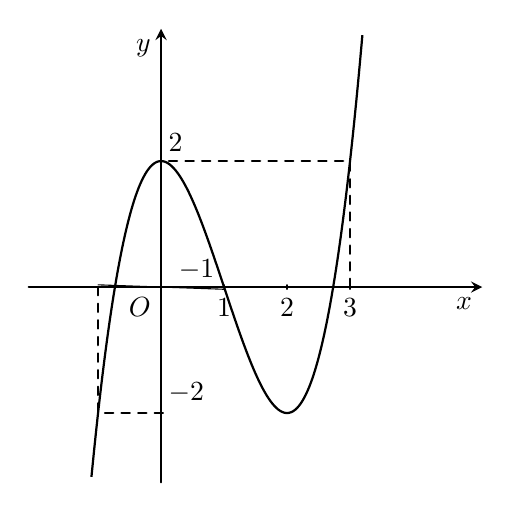
\begin{tikzpicture}[line join=round, line cap=round,>=stealth,thick,scale=.8]
			\tikzset{label style/.style={font=\footnotesize}}
			\draw[->] (-2.1,0)--(5.1,0) node[below left] {$x$};
			\draw[->] (0,-3.1)--(0,4.1) node[below left] {$y$};
			\draw (0,0) node [below left] {$O$};
			\foreach \x in {1,2,3}
			\draw[thin] (\x,1pt)--(\x,-1pt) node [below] {$\x$};
			\draw[thin](-1,1pt)--(1,-1pt)node[above left]{$-1$};
			\foreach \y in {-2,2}
			\draw[thin] (1pt,\y)--(-1pt,\y) node [above right] {$\y$};
			%\begin{scope}
			\clip (-2,-3) rectangle (5,4);
			\draw[samples=200,domain=-2:4,smooth,variable=\x] plot (\x,{(\x)^3-3*(\x)^2+2});
			%\end{scope}
			\draw[dashed] (-1,0)--(-1,-2)--(0,-2);
			\draw[dashed] (3,0)--(3,2)--(0,2);
			%\begin{scope}[on background layer]\path[white]node{MDD-134};\end{scope}
		\end{tikzpicture}
	}
	\loigiai
	{
		\immini{Xét hàm số $g(x)=f(3 x+1)+9 x^3+\dfrac{9}{2}x^2 \\
			\Rightarrow g'(x)=3 f'(3 x+1)+27 x^2+9 x$.\\
			Hàm số đồng biến  $\Leftrightarrow g'(x)>0 \Leftrightarrow 3 f'(3 x+1)+27 x^2+9 x>0$
			\\
			$
			\Leftrightarrow f'(3 x+1)+3 x(3 x+1)>0 \qquad (*)
			$\\
			Đặt $t=3 x+1$, khi đó  $(*) \Leftrightarrow f'(t)+(t-1) t>0$\\ $\Leftrightarrow f'(t)>-t^2+t$.\\
			Vẽ parabol $y=-x^2+x$ và đồ thị hàm số $f'(x)$ trên cùng một hệ trục
		}
		{
			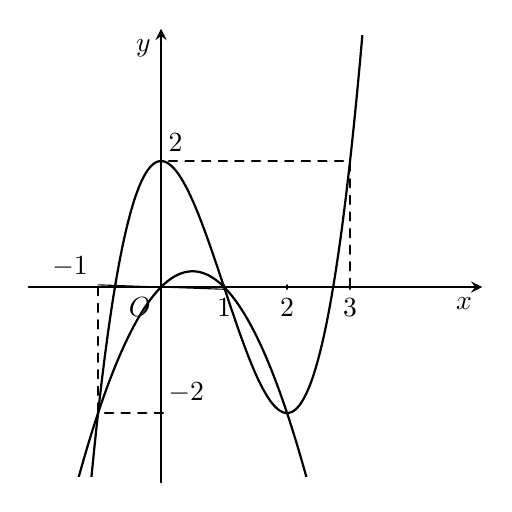
\begin{tikzpicture}[line join=round, line cap=round,>=stealth,thick,scale=.8]
				\tikzset{label style/.style={font=\footnotesize}}
				\draw[->] (-2.1,0)--(5.1,0) node[below left] {$x$};
				\draw[->] (0,-3.1)--(0,4.1) node[below left] {$y$};
				\draw (0,0) node [below left] {$O$};
				\foreach \x in {1,2,3}
				\draw[thin] (\x,1pt)--(\x,-1pt) node [below] {$\x$};
				\draw[thin](-1,1pt)--(1,-1pt);
				\foreach \y in {-2,2}
				\draw[thin] (1pt,\y)--(-1pt,\y) node [above right] {$\y$};
				%\begin{scope}
				\clip (-2,-3) rectangle (5,4);
				\draw[samples=200,domain=-2:4,smooth,variable=\x] plot (\x,{(\x)^3-3*(\x)^2+2});
				\draw[samples=200,domain=-2:4,smooth,variable=\x] plot (\x,{-(\x)^2+(\x)});
				%\end{scope}
				\draw[dashed] (-1,0) node[above left]{$-1$}--(-1,-2)--(0,-2);
				\draw[dashed] (3,0)--(3,2)--(0,2);
				%\begin{scope}[on background layer]\path[white]node{MDD-134};\end{scope}
			\end{tikzpicture}
		}
		Dựa vào đồ thị ta thấy
		$
		f'(t)>-t^2+t \Leftrightarrow\hoac{&- 1 < t < 1\\
			&t > 2}\Rightarrow \hoac{&
			- 1 < 3 x + 1 < 1\\
			&3 x + 1 > 2} \Leftrightarrow \hoac{&
			\dfrac{-2}{3}<x<0\\
			&x>\dfrac{1}{3}.}
		$}
\end{ex}
\begin{ex}[Sở Phú Thọ-2020]%[2D1G1-2]
	\immini{
		Cho hàm số $y=f(x)$ có đồ thị hàm số $y=f'(x)$ như hình vẽ.\\
		Hàm số $g(x)=f\left(\mathrm{e}^x-2\right)-2020$ nghịch biến trên khoảng nào dưới đây?
		\choice
		{\True $\left(-1 ; \dfrac{3}{2}\right)$}
		{$(-1 ; 2)$}
		{$(0 ;+\infty)$}
		{$\left(\dfrac{3}{2}; 2\right)$}
	}
	{
		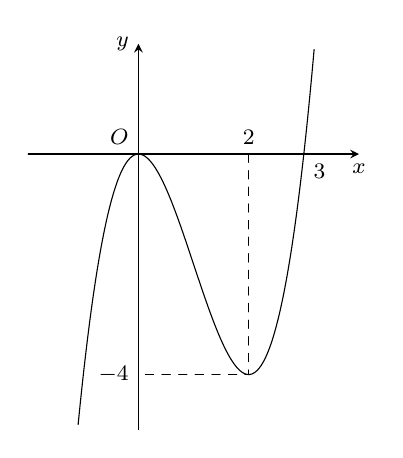
\begin{tikzpicture}[scale=0.7,>=stealth, font=\footnotesize, line join=round, line cap=round]
			\def\a{1} \def\b{-3} \def\c{0} \def\d{0} % Hệ số
			\def\xmin{-2} \def\xmax{4}
			\def\ymin{-5} \def\ymax{2} 
			%\draw[color=gray!50,dashed] (\xmin,\ymin) grid (\xmax,\ymax); 
			\draw[->] (\xmin,0)--(\xmax,0) node [below]{$x$};
			\draw[->] (0,\ymin)--(0,\ymax) node [left]{$y$};
			\node at (0,0) [above left]{$O$};
			\node at (3,0) [below right]{$3$};
			\draw[dashed] (2,0) node[above]{$2$}--(2,-4) --(0,-4) node[left]{$-4$};
			\clip (\xmin+0.1,\ymin+0.1) rectangle (\xmax-0.5,\ymax-0.1);
			\draw[smooth,samples=300] plot(\x,{\a*(\x)^3+\b*(\x)^2+\c*(\x)+\d});
		\end{tikzpicture}
	}
	
	\loigiai{
		Dựa vào đồ thị hàm số $y=f'(x)$ suy ra $f'(x) \leq 0 ~ \forall x<3$ và $f'(x)>0 ~ \forall x>3$.
		$
		g'(x)=\mathrm{e}^x f'\left(\mathrm{e}^x-2\right) .
		$
		Hàm số $g(x)=f\left(\mathrm{e}^x-2\right)-2020$ nghịch biến \\ $ \Leftrightarrow g'(x)<0 \Leftrightarrow \mathrm{e}^x f'\left(\mathrm{e}^x-2\right)<0$\\
		$
		\Leftrightarrow f'\left(\mathrm{e}^x-2\right)<0 \Leftrightarrow \mathrm{e}^x-2<3 \Leftrightarrow \mathrm{e}^x<5 \Leftrightarrow x<\ln 5 .
		$\\
		Vậy hàm số đã cho nghịch biến trên $\left(-1 ; \dfrac{3}{2}\right)$.
	}
\end{ex}
\begin{ex}[Lý Nhân Tông - Bắc Ninh - 2020]%[2D1G1-2]
	\immini{
		Cho hàm số $f(x)$ có đồ thị hàm số $f'(x)$ như hình vẽ.\\
		Hàm số $y=f(\cos x)+x^2-x$ đồng biến trên khoảng
		\choice
		{$(-2 ; 1)$}
		{$(0 ; 1)$}
		{\True $(1 ; 2)$}
		{$(-1 ; 0)$}
	}
	{
		\begin{tikzpicture}[scale=1,>=stealth, font=\footnotesize, line join=round, line cap=round]
			\def\a{-0.5} \def\b{0} \def\c{1.5} \def\d{0} % Hệ số
			\def\xmin{-3} \def\xmax{4}
			\def\ymin{-2} \def\ymax{2} 
			%\draw[color=gray!50,dashed] (\xmin,\ymin) grid (\xmax,\ymax); 
			\draw[->] (\xmin,0)--(\xmax,0) node [below]{$x$};
			\draw[->] (0,\ymin)--(0,\ymax) node [left]{$y$};
			\node at (0,0) [above left]{$O$};
			\node at (3,0) [below right]{$3$};
			\draw[dashed] (-2,0) node[below]{$-2$}--(-2,1) --(0,1) node[above right]{$1$} --(1,1)--(1,0) node[below]{$1$};
			\draw[dashed] (-1,0) node[below right]{$-1$}--(-1,-1) --(0,-1) node[above right]{$-1$} --(2,-1)--(2,0) node[below right]{$2$};
			\clip (\xmin+0.1,\ymin+0.1) rectangle (\xmax-0.5,\ymax-0.1);
			\draw[smooth,samples=300][domain=-2:2] plot(\x,{\a*(\x)^3+\b*(\x)^2+\c*(\x)+\d});
		\end{tikzpicture}
	}
	\loigiai{
		Đặt  $g(x)=f(\cos x)+x^2-x$.\\
		Ta có $g'(x)=-\sin x \cdot f'(\cos x)+2 x-1$\\
		Vì $\cos x \in[-1 ; 1]$ nên từ đồ thị $f'(x)$ ta suy ra $f'(\cos x) \in[-1 ; 1]$.\\
		Do đó $\left|-\sin x \cdot f'(\cos x)\right| \leq 1, ~\forall x \in \mathbb{R}$.\\
		Ta suy ra $g'(x)=\sin x \cdot f'(\cos x)+2 x-1 \geq-1+2 x-1=2 x-2$
		$\Rightarrow g'(x)>0, ~\forall x>1$.\\
		Vậy hàm số đồng biến trên $(1 ; 2)$.
	}
\end{ex}
\begin{ex}[THPT Nguyễn Viết Xuân - 2020]%[2D1G1-2]
	\immini{
		Cho hàm số $f(x)$. Hàm số $y=f'(x)$ có đồ thị như hình vẽ.\\
		Hàm số $g(x)=f\left(3 x^2-1\right)-\dfrac{9}{2}x^4+3 x^2$ đồng biến trên khoảng nào dưới đây?
		\choice
		{\True $\left(-\dfrac{2 \sqrt{3}}{3}; \dfrac{-\sqrt{3}}{3}\right)$}
		{$\left(0 ; \dfrac{2 \sqrt{3}}{3}\right)$}
		{$(1 ; 2)$}
		{$\left(-\dfrac{\sqrt{3}}{3}; \dfrac{\sqrt{3}}{3}\right)$} 
	}
	{
		\begin{tikzpicture}[scale=0.6,>=stealth, font=\footnotesize, line join=round, line cap=round]
			\def\a{0.25} \def\b{0.25} \def\c{-2} \def\d{0} % Hệ số
			\def\xmin{-5} \def\xmax{4}
			\def\ymin{-5} \def\ymax{5} 
			%\draw[color=gray!50,dashed] (\xmin,\ymin) grid (\xmax,\ymax); 
			\draw[->] (\xmin,0)--(\xmax,0) node [below]{$x$};
			\draw[->] (0,\ymin)--(0,\ymax) node [left]{$y$};
			\node at (0,0) [above left]{$O$};
			%\node at (3,0) [below right]{$3$};
			\draw[dashed] (-4,0) node[below left]{$-4$}--(-4,-4) --(0,-4) node[above right]{$-4$};
			\draw[dashed] (3,0) node[below right]{$3$}--(3,3) --(0,3) node[above right]{$3$};
			\clip (\xmin+0.1,\ymin+0.1) rectangle (\xmax-0.5,\ymax-0.1);
			\draw[smooth,samples=300] plot(\x,{\a*(\x)^3+\b*(\x)^2+\c*(\x)+\d});
		\end{tikzpicture}
	}
	
	\loigiai
	{
		TXĐ: $\mathscr{D}=\mathbb{R}$.\\
		Ta có $g'(x)=6 x f'\left(3 x^2-1\right)-18 x^3+6 x=6 x\left[f'\left(3 x^2-1\right)-3 x^2+1\right]$.\\
		$
		g'(x)=0 \Leftrightarrow\hoac{
			&x = 0\\
			&f '( 3 x ^{2}- 1 ) = 3 x ^{2}- 1}
		\Leftrightarrow \hoac{
			&x = 0\\
			&3 x ^{2}- 1 = - 4 \text{~(vô nghiệm)}\\
			&3 x ^{2}- 1 = 0\\
			&3 x ^{2}- 1 = 3}\Leftrightarrow \hoac{&x=0 \\
			&x=\pm \dfrac{\sqrt{3}}{3}\\
			&x=\pm \dfrac{2 \sqrt{3}}{3}.}
		$\\
		Bảng xét dấu
		\begin{center}
			
\begin{tikzpicture}
				\tkzTabInit[nocadre,lgt=1.2,espcl=2.2,deltacl=0.6]
				{$x$ /1.2,$f'(x)$ /0.7}
				{$-\infty$,$-\dfrac{2 \sqrt{3}}{3}$,$-\dfrac{ \sqrt{3}}{3}$,$0$,$\dfrac{\sqrt{3}}{3}$,$\dfrac{2 \sqrt{3}}{3}$,$+\infty$}
				\tkzTabLine{,-,$0$,+,$0$,-,$0$,+,$0$,-,$0$,+,}
			\end{tikzpicture}
		\end{center}
		Vậy hàm số đồng biến trong khoảng $\left(-\dfrac{2 \sqrt{3}}{3}; \dfrac{-\sqrt{3}}{3}\right)$.}
\end{ex}
\begin{ex}[Trần Phú - Quảng Ninh - 2020]%[2D1G1-2]
	Cho hàm số $f(x)$ có bảng xét dấu của đạo hàm như sau
	\begin{center}
		
\begin{tikzpicture}
			\tkzTabInit[nocadre,lgt=1.2,espcl=2,deltacl=0.6]
			{$x$ /0.6,$f'(x)$ /0.6}
			{$-\infty$,$-4$,$-1$,$2$,$7$,$+\infty$}
			\tkzTabLine{,+,$0$,-,$0$,+,$0$,-,$0$,+,}
		\end{tikzpicture}
	\end{center}
	Hàm số $y=f(2 x+1)+\dfrac{2}{3}x^3-8 x+5$ nghịch biến trên khoảng nào dưới đây?
	\choice
	{$(-\infty ;-2)$}
	{$(1 ;+\infty)$}
	{$(-1 ; 7)$}
	{\True $\left(-1 ; \dfrac{1}{2}\right)$}
	\loigiai{
		Ta có $y'=2 f'(2 x+1)+2 x^2-8$.\\
		Xét $y'\leq 0 \Leftrightarrow 2 f'(2 x+1)+2 x^2-8 \leq 0 \Leftrightarrow f'(2 x+1) \leq 4-x^2$.\\
		Đặt $t=2x+1$, ta có $f'(t) \leq \dfrac{-t^2+2 t+15}{4}$.\\
		Vì $\dfrac{-t^2+2 t+15}{4}\geq 0, \forall t \in[-3 ; 5]$.\\
		Mà $f'(t) \leq 0, \forall t \in[-3 ; 2]$.\\
		Nên $f'(t) \leq \dfrac{-t^2+2 t+15}{4}\Rightarrow t \in[-3 ; 2]$.\\
		Suy ra $-3 \leq 2 x+1 \leq 2 \Leftrightarrow-2 \leq x \leq \dfrac{1}{2}$.}
\end{ex}

\begin{ex}[Chuyên Thái Bình - Lần 3 - 2020]%[2D1G1-2]
	\immini{
		Cho hàm số $y=f(x)$ liên tục trên $\mathbb{R}$ có đồ thị hàm số $y=f'(x)$ cho như hình vẽ.\\
		Hàm số $g(x)=2 f(|x-1|)-x^2+2 x+2020$ đồng biến trên khoảng nào?
		\choice
		{\True $(0 ; 1)$}
		{$(-3 ; 1)$}
		{$(1 ; 3)$}
		{$(-2 ; 0)$}
	}
	{
		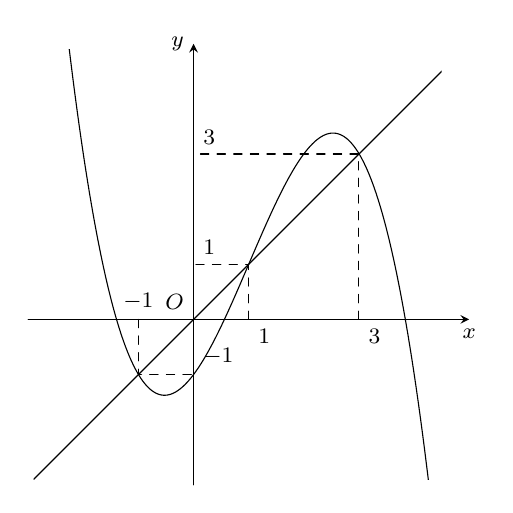
\begin{tikzpicture}[scale=0.7,>=stealth, font=\footnotesize, line join=round, line cap=round]
			\def\a{-0.333} \def\b{1} \def\c{1.333} \def\d{-1} % Hệ số
			\def\xmin{-3} \def\xmax{5}
			\def\ymin{-3} \def\ymax{5} 
			%\draw[color=gray!50,dashed] (\xmin,\ymin) grid (\xmax,\ymax); 
			\draw[->] (\xmin,0)--(\xmax,0) node [below]{$x$};
			\draw[->] (0,\ymin)--(0,\ymax) node [left]{$y$};
			\node at (0,0) [above left]{$O$};
			%\node at (3,0) [below right]{$3$};
			\draw[dashed] (-1,0) node[above]{$-1$}--(-1,-1) --(0,-1) node[above right]{$-1$};
			\draw[dashed] (1,0) node[below right]{$1$}--(1,1) --(0,1) node[above right]{$1$};
			\draw[dashed] (3,0) node[below right]{$3$}--(3,3) --(0,3) node[above right]{$3$};
			\clip (\xmin+0.1,\ymin+0.1) rectangle (\xmax-0.5,\ymax-0.1);
			\draw[smooth,samples=300] plot(\x,{\a*(\x)^3+\b*(\x)^2+\c*(\x)+\d});
			\draw[smooth,samples=300] plot(\x,{(\x)});
		\end{tikzpicture}
	}
	\loigiai{
		Với $x>1$, ta có $g(x)=2 f(x-1)-(x-1)^2+2021 \Rightarrow g'(x)=2 f'(x-1)-2(x-1)$.\\
		Hàm số đồng biến $\Leftrightarrow 2 f'(x-1)-2(x-1)>0 \Leftrightarrow f'(x-1)>x-1 \quad(*)$.\\
		Đặt $t=x-1$, khi đó $(*) \Leftrightarrow f'(t)>t \Leftrightarrow\hoac{&1<t<3 \\ &t<-1}\Rightarrow\hoac{&2<x<4 \\ &x<0 ~(\text{loại}).}$\\
		Với $x<1$, ta có $g(x)=2 f(1-x)-(1-x)^2+2021 \Rightarrow g'(x)=-2 f'(1-x)+2(1-x)$.\\
		Hàm số đồng biến $\Leftrightarrow-2 f'(1-x)+2(1-x)>0 \Leftrightarrow f'(1-x)<1-x \quad(* *)$.\\
		Đặt $t=1-x$, khi đó $(* *) \Leftrightarrow f'(t)<t \Leftrightarrow\hoac{&-1<t<1 \\ &t>3}\Rightarrow\hoac{&0<x<2 \\ &x<-2}\Rightarrow\hoac{&0<x<1 \\ &x<-2.}$\\
		Vậy hàm số $g(x)$ đồng biến trên các khoảng $(-\infty ;-2),(0 ; 1),(2 ; 4)$.
	}
\end{ex}
\begin{ex}[Sở Phú Thọ - 2020]%[2D1G1-2]
	\immini{
		Cho hàm số $y=f(x)$ có đồ thị hàm số $f'(x)$ như hình vẽ.\\
		Hàm số $g(x)=f\left(1+e^x\right)+2020$ nghịch biến trên khoảng nào dưới đây?
		\choice
		{$(0 ;+\infty)$}
		{$\left(\dfrac{1}{2}; 1\right)$}
		{\True $\left(0 ; \dfrac{1}{2}\right)$}
		{$(-1 ; 1)$}
	}{
		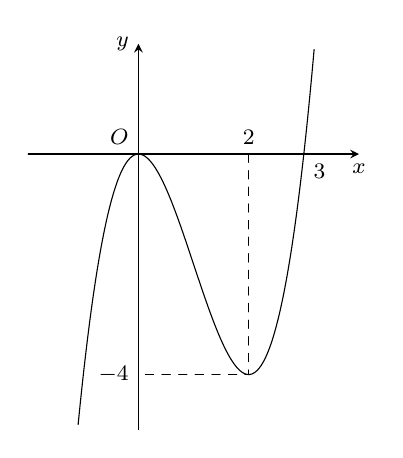
\begin{tikzpicture}[scale=0.7,>=stealth, font=\footnotesize, line join=round, line cap=round]
			\def\a{1} \def\b{-3} \def\c{0} \def\d{0} % Hệ số
			\def\xmin{-2} \def\xmax{4}
			\def\ymin{-5} \def\ymax{2} 
			%\draw[color=gray!50,dashed] (\xmin,\ymin) grid (\xmax,\ymax); 
			\draw[->] (\xmin,0)--(\xmax,0) node [below]{$x$};
			\draw[->] (0,\ymin)--(0,\ymax) node [left]{$y$};
			\node at (0,0) [above left]{$O$};
			\node at (3,0) [below right]{$3$};
			\draw[dashed] (2,0) node[above]{$2$}--(2,-4) --(0,-4) node[left]{$-4$};
			\clip (\xmin+0.1,\ymin+0.1) rectangle (\xmax-0.5,\ymax-0.1);
			\draw[smooth,samples=300] plot(\x,{\a*(\x)^3+\b*(\x)^2+\c*(\x)+\d});
		\end{tikzpicture}
	}
	\loigiai{
		$g'(x)=e^x f'\left(1+e^x\right)$.\\
		Do $e^x>0, \forall x$ nên $g'(x) \leq 0 \Leftrightarrow f'\left(1+e^x\right) \leq 0 \Leftrightarrow 1+e^x \leq 3 \Leftrightarrow x \leq \ln 2$, dấu bằng xảy ra tại hữu hạn điểm.\\
		Nên $g(x)$ nghịch biến trên $(-\infty ; \ln 2)$.\\
		Vì $\left(0 ; \dfrac{1}{2}\right) \subset (-\infty ; \ln 2)$ nên hàm số đã cho nghịch biến trên $\left(0 ; \dfrac{1}{2}\right)$.
	}
\end{ex}

\begin{ex}%[2D1K1-2]
	[THPT Anh Sơn - Nghệ An - 2020]
	Cho hàm số $y=f(x)$ có bảng xét dấu của đạo hàm như sau.
	\begin{center}
		
\begin{tikzpicture}
			\tkzTabInit[nocadre,lgt=1.2,espcl=2,deltacl=0.6]
			{$x$ /0.6,$f'(x)$ /0.6}
			{$-\infty$,$-2$,$-1$,$2$,$4$,$+\infty$}
			\tkzTabLine{,+,$0$,-,$0$,+,$0$,-,$0$,+,}
		\end{tikzpicture}
	\end{center}
	Hàm số $y=-2 f(x)+2019$ nghịch biến trên khoảng nào trong các khoảng dưới đây?
	\choice
	{$(2 ; 4)$}
	{$(-4 ; 2)$}
	{$(-2 ;-1)$}
	{\True $(-1 ; 2)$}
	\loigiai{
		Ta có $y'=-2 f'(x)$.\\
		$
		y'=0 \Leftrightarrow-2 f'(x)=0 \Leftrightarrow\hoac{&
			x=-2 \\
			&x=-1 \\
			&x=2 \\
			&x=4.}$\\
		Từ bảng xét dấu của $f'(x)$ ta có
		\begin{center}
			
\begin{tikzpicture}
				\tkzTabInit[nocadre,lgt=1,espcl=2,deltacl=0.6]
				{$x$ /0.6,$y'$ /0.6}
				{$-\infty$,$-2$,$-1$,$2$,$4$,$+\infty$}
				\tkzTabLine{,-,$0$,+,$0$,-,$0$,+,$0$,-,}
			\end{tikzpicture}
		\end{center}
		Từ bảng xét dấu ta có hàm số nghịch biến trên khoảng $(-\infty ;-2),(-1 ; 2)$ và $(4 ;+\infty)$.}
\end{ex}

\begin{ex}[THPT Anh Sơn - Nghệ An - 2020]%[2D1G1-2]
	Cho hàm số $f(x)$ xác định và liên tục trên $\mathbb{R}$ và có đạo hàm $f'(x)$ thỏa mãn $f'(x)=(1-x)(x+2) g(x)+2019$ với $g(x)<0, ~\forall x \in \mathbb{R}$ . Hàm số $y=f(1-x)+2019 x+2020$ nghịch biến trên khoảng nào?
	\choice
	{$(1 ;+\infty)$}
	{$(0 ; 3)$}
	{$(-\infty ; 3)$}
	{\True $(3 ;+\infty)$}
	\loigiai{
		Đặt $h(x)=f(1-x)+2019 x+2020$.\\
		Vì hàm số $f(x)$ xác định trên $\mathbb{R}$ nên hàm số $h(x)$ cũng xác định trên $\mathbb{R}$.\\
		Ta có $h'(x)=-f'(1-x)+2019$.\\
		Do $h'(x)=0$ tại hữu hạn điểm nên để tìm khoảng nghịch biến của hàm số $h(x)$, ta tìm các giá trị của $x$ sao cho $h'(x)<0 \Leftrightarrow-f'(1-x)+2019<0$\\ 
		$\Leftrightarrow f'(1-x)-2019>0 \\
		\Leftrightarrow x(3-x) g(1-x)>0 \Leftrightarrow x(3-x)<0(\text{~do~}g(x)<0, \forall x \in \mathbb{R})$\\
		$\Leftrightarrow\hoac{&
			x<0 \\
			&x>3.}$\\
		Vậy hàm số $y=f(1-x)+2019 x+2020$ nghịch biến trên các khoảng $(-\infty ; 0)$ và $(3 ;+\infty).$}
\end{ex}

\begin{ex}%[2D1G1-2]
	Cho hàm số $y=f(x)$ xác định trên $\mathbb{R}$ và có bảng xét dấu đạo hàm như sau:
	\begin{center}
		
\begin{tikzpicture}
			\tkzTabInit[nocadre,lgt=2,espcl=2,deltacl=0.6]
			{$x$ /0.6,$f'(x)$ /0.6}
			{$-\infty$,$-1$,$1$,$4$,$+\infty$}
			\tkzTabLine{,-,$0$,+,$0$,-,$0$,+,}
		\end{tikzpicture}
	\end{center}
	Biết $f(x)>2,~ \forall x \in \mathbb{R}$. Xét hàm số $g(x)=f(3-2 f(x))-x^3+3 x^2-2020$. Khẳng định nào sau đây đúng?
	\choice
	{Hàm số $g(x)$ đồng biến trên khoảng $(-2 ;-1)$}
	{Hàm số $g(x)$ nghịch biến trên khoảng $(0 ; 1)$}
	{Hàm số $g(x)$ đồng biến trên khoảng $(3 ; 4)$}
	{\True Hàm số $g(x)$ nghịch biến trên khoảng $(2 ; 3)$}
	\loigiai{
		Ta có $g'(x)=-2 f'(x) f'(3-2 f(x))-3 x^2+6 x$.\\
		Vì $f(x)>2, ~\forall x \in \mathbb{R}$ nên $3-2 f(x)<-1 ~\forall x \in \mathbb{R}$.\\
		Từ bảng xét dấu $f'(x)$ suy ra $f'(3-2 f(x))<0, ~\forall x \in \mathbb{R}$.\\
		Từ đó ta có bảng xét dấu sau:
		\begin{center}
			\begin{tikzpicture}
				\tkzTabInit[nocadre,lgt=4,espcl=1.7,deltacl=0.6]
				{$x$ /0.7,$-f'(x)f'\left( 3-2f(x)\right) $/0.8,$-3x^2+6x$/0.7}
				{$-\infty$,$-1$,$0$,$1$,$2$,$4$,$+\infty$}
				\tkzTabLine{,-,$0$,+,|,+,$0$,-,|,-,$0$,+,}
				\tkzTabLine{,-,|,-,$0$,+,|,+,$0$,-,|,-,}
			\end{tikzpicture}
		\end{center}
		Từ bảng xét dấu trên, loại trừ đáp án suy ra hàm số $g(x)$ nghịch biến trên khoảng $(2 ; 3)$.}
\end{ex}

\begin{ex}%[2D1G1-2]
	Cho hàm số $f(x)$ có bảng biến thiên như sau:
	\begin{center}
		
\begin{tikzpicture}
			\tkzTabInit[nocadre,lgt=1.2,espcl=2.5,deltacl=0.6]
			{$x$ /0.7, $f'(x)$ /0.7, $f(x)$ /2.5}
			{$-\infty$,$1$,$2$,$3$,$4$,$+\infty$}
			\tkzTabLine{,+,$0$,-,$0$,+,$0$,-,$0$,+,}
			\tkzTabVar{-/$-\infty$,+/$3$,-/$1$,+/$2$,-/$0$,+/$+\infty$}
		\end{tikzpicture}
	\end{center}
	Hàm số $y=(f(x))^3-3 .(f(x))^2$ nghịch biến trên khoảng nào dưới đây?
	\choice
	{$(1 ; 2)$}
	{$(3 ; 4)$}
	{$(-\infty ; 1)$}
	{\True $(2 ; 3)$}
	\loigiai{
		Ta có $y'=3 \cdot(f(x))^2 \cdot f'(x)-6 \cdot f(x) \cdot f'(x)=3 f(x) \cdot f'(x) \cdot[f(x)-2]. \\
		y'=0 \Leftrightarrow \hoac{&f(x)=0 \Leftrightarrow x \in\left\{x_1, 4 \mid x_1<1\right\}\\
			&f(x)=2 \Leftrightarrow x \in\left\{x_2, x_3, 3, x_4 \mid x_1<x_2<1<x_3<2 ; 4<x_4\right\}\\
			&f'(x)=0 \Leftrightarrow x \in\{1,2,3,4\}.}$\\
		Lập bảng xét dấu ta có
		\begin{center}
			
\begin{tikzpicture}
				\tkzTabInit[nocadre,lgt=2,espcl=1.5,deltacl=0.6]
				{$x$ /0.7,$f(x)$ /0.7,$f(x)-2$ /0.7,$f'(x)$/0.7,$y'$/0.7}
				{$-\infty$,$x_1$,$x_2$,$1$,$x_3$,$2$,$3$,$4$,$x_4$,$+\infty$}
				\tkzTabLine{,-,$0$,+,|,+,|,+,|,+,|,+,$0$,+,|,+,|,+,}
				\tkzTabLine{,-,|,-,$0$,+,$0$,+,$0$,-,|,-,$0$,-,|,-,$0$,+}
				\tkzTabLine{,+,|,+,|,+,$0$,-,|,-,$0$,+,$0$,-,$0$,+,|,+}
				\tkzTabLine{,+,$0$,-,$0$,+,$0$,-,$0$,+,$0$,-,$0$,+,$0$,-,$0$,+}
			\end{tikzpicture}
		\end{center}
		
		Do đó hàm số nghịch biến trên khoảng $(2 ; 3)$.
	}
\end{ex}
\begin{ex}%[2D1G1-2]
	Cho hàm số $y=f(x)$ có đồ thị nằm trên trục hoành và có đạo hàm trên $\mathbb{R}$, bảng xét dấu của biểu thức $f'(x)$ như bảng dưới đây.
	\begin{center}
		
\begin{tikzpicture}
			\tkzTabInit[nocadre,lgt=1.2,espcl=2,deltacl=0.6]
			{$x$ /0.6,$f'(x)$ /0.6}
			{$-\infty$,$-2$,$-1$,$3$,$+\infty$}
			\tkzTabLine{,-,$0$,+,$0$,-,$0$,+,}
		\end{tikzpicture}
	\end{center}
	Hàm số $y=g(x)=\dfrac{f\left(x^2-2 x\right)}{f\left(x^2-2 x\right)+1}$ nghịch biến trên khoảng nào dưới đây?
	\choice
	{$(-\infty ; 1)$}
	{$\left(-2 ; \dfrac{5}{2}\right)$}
	{\True $(1 ; 3)$}
	{$(2 ;+\infty)$}
	\loigiai{
		$ g'(x)=\dfrac{\left(x^2-2 x\right)'\cdot f'\left(x^2-2 x\right)}{\left(f\left(x^2-2 x\right)+1\right)^2}=\dfrac{(2 x-2) \cdot f'\left(x^2-2 x\right)}{\left(f\left(x^2-2 x\right)+1\right)^2}. \\
		g'(x)=0 \Leftrightarrow\hoac{
			&2 x - 2 = 0\\
			&f '( x ^{2}- 2 x ) = 0}
		\Leftrightarrow \hoac{&x = 1\\
			&x ^{2}- 2 x = - 2\\
			&x ^{2}- 2 x = - 1\\
			&x ^{2}- 2 x = 3}
		\Leftrightarrow \hoac{&x=1 \\
			&x=-1 \\
			&x=3.}
		$\\
		Ta có bảng xét dấu của $g'(x)$
		\begin{center}
			
\begin{tikzpicture}
				\tkzTabInit[nocadre,lgt=1.2,espcl=2,deltacl=0.6]
				{$x$ /0.6,$g'(x)$ /0.6}
				{$-\infty$,$-1$,$1$,$3$,$+\infty$}
				\tkzTabLine{,-,$0$,+,$0$,-,$0$,+,}
			\end{tikzpicture}
		\end{center}
		Dựa vào bảng xét dấu ta có hàm số $y=g(x)$ nghịch biến trên các khoảng $(-\infty ;-1)$ và $(1 ; 3)$.}
\end{ex}
\begin{ex}[Liên trường huyện Quảng Xương - Thanh Hóa - 2021]%[2D1G1-2]
	\immini{
		Cho các hàm số $y=f(x)$; $y=g(x)$ liên tục trên $\mathbb{R}$ và có đồ thị các đạo hàm $f'(x) ; g'(x)$ (đồ thị hàm số $y=g'(x)$ là đường đậm hơn) như hình vẽ.\\
		Hàm số $h(x)=f(x-1)-g(x-1)$ nghịch biến trên khoảng nào dưới đây?
		\choice
		{$\left(\dfrac{1}{2}; 1\right)$}
		{$(1 ;+\infty)$}
		{$(2 ;+\infty)$}
		{\True $\left(-1 ; \dfrac{1}{2}\right)$}
	}
	{
		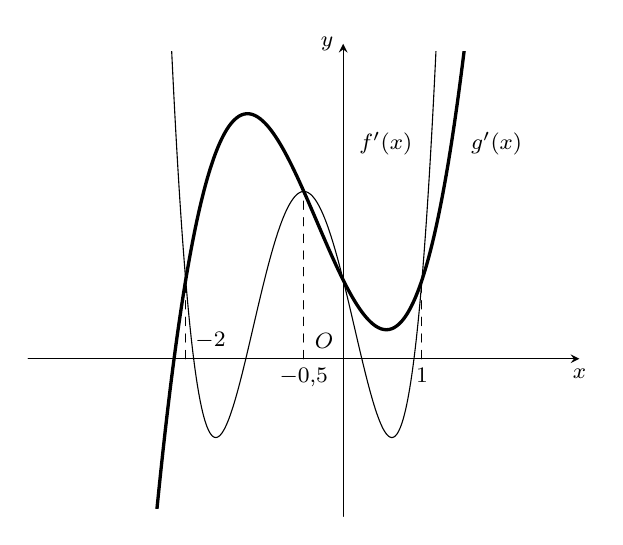
\begin{tikzpicture}[scale=1,>=stealth, font=\footnotesize, line join=round, line cap=round]
			%\def\a{1} \def\b{-6} \def\c{9} \def\d{1} % Hệ số
			\def\xmin{-4} \def\xmax{3}
			\def\ymin{-2} \def\ymax{4} 
			%\draw[color=gray!50,dashed] (\xmin,\ymin) grid (\xmax,\ymax); 
			\draw[->] (\xmin,0)--(\xmax,0) node [below]{$x$};
			\draw[->] (0,\ymin)--(0,\ymax) node [left]{$y$};
			\node at (0,0) [above left]{$O$};
			\node at (1,3) [below left]{$f'(x)$};
			\node at (1.5,3) [below right]{$g'(x)$};
			\draw[dashed] (-2,0) node[above right]{$-2$}--(-2,1);
			\draw[dashed] (1,0) node[below]{$1$}--(1,1);
			\draw[dashed] (-0.5,0) node[below]{$-0{,}5$}--(-0.5,2.125);
			\clip (\xmin+0.1,\ymin+0.1) rectangle (\xmax-0.5,\ymax-0.1);
			\draw[smooth,samples=300][domain=-3:2] plot(\x,{2*(\x)^4+4*(\x)^3-2*(\x)^2-4*(\x)+1});
			\draw[smooth,samples=300,line width=1.2pt] plot(\x,{(\x)^3+(\x)^2-2*(\x)+1});
		\end{tikzpicture}
	}
	
	\loigiai{
		Ta có: $h'(x)=f'(x-1)-g'(x-1)$.\\
		Dựa vào hình vẽ ta có hàm số $h(x)$ nghịch biến\\
		$\Leftrightarrow h'(x)<0 \Leftrightarrow f'(x-1)<g'(x-1)$\\
		$
		\Leftrightarrow\hoac{&- 2 < x - 1 < - \dfrac{1}{2}\\
			&0 < x - 1 < 1}
		\Leftrightarrow \hoac{
			&-1<x<\dfrac{1}{2}\\
			&1<x<2.}$\\
		Do đó hàm số $h(x)$ nghịch biến trên các khoảng $\left(-1 ; \dfrac{1}{2}\right)$ và $(1 ; 2)$.
	}
\end{ex}
\begin{ex}[THPT Quế Võ 1 - Bắc Ninh - 2021] %[2D1G1-2]
	\immini{
		Cho ba hàm số $y=f(x), y=g(x), y=h(x)$. Đồ thị của ba hàm số $y=f'(x), y=g'(x), y=h'(x)$ được cho như hình vẽ.\\
		Hàm số $k(x)=f(x+7)+g(5 x+1)-h\left(4 x+\dfrac{3}{2}\right)$ đồng biến trên khoảng nào dưới đây?
		\choice
		{$\left(-\dfrac{5}{8}; 0\right)$}
		{$\left(\dfrac{5}{8};+\infty\right)$}
		{\True $\left(\dfrac{3}{8}; 1\right)$}
		{$\left(-\dfrac{3}{8}; 1\right)$}
	}
	{
		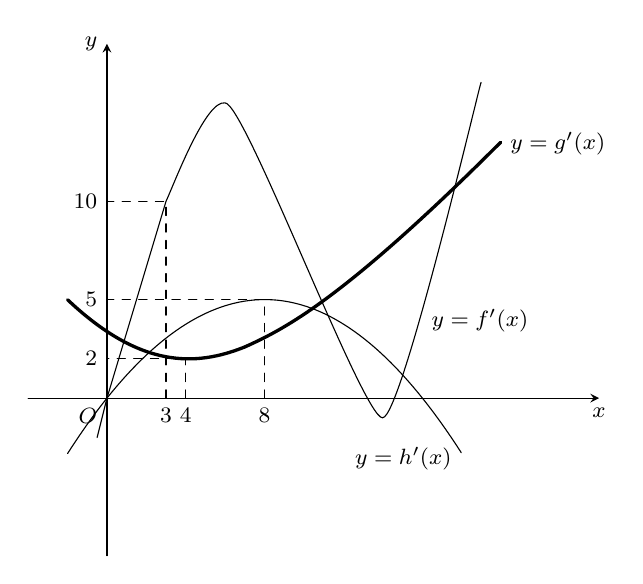
\begin{tikzpicture}[scale=0.25,>=stealth, font=\footnotesize, line join=round, line cap=round]
			\def\a{-.078} \def\b{1.25} \def\c{0} % Hệ số
			\def\xmin{-4} \def\xmax{25}
			\def\ymin{-8} \def\ymax{18}
			
			%\draw[color=gray!50,dashed] (\xmin,\ymin) grid (\xmax,\ymax);
			
			\draw[->] (\xmin,0)--(\xmax,0) node [below]{$x$};
			\draw[->] (0,\ymin)--(0,\ymax) node [left]{$y$};
			\node at (20,14) [below right]{$y=g'(x)$};
			\node at (18,-2) [below left]{$y=h'(x)$};
			\node at (16,5) [below right]{$y=f'(x)$};
			\node at (0,0) [below left]{$O$};
			\draw[dashed] (3,0) node[below]{$3$}--(3,10)--(0,10) node[left]{$10$};
			\draw[dashed] (8,0) node[below]{$8$}--(8,5)--(0,5) node[left]{$5$};
			\draw[dashed] (4,0) node[below]{$4$}--(4,2)--(0,2) node[left]{$2$};
			\clip (\xmin+0.1,\ymin+0.1) rectangle (\xmax-0.5,\ymax-0.1);
			\draw[smooth,samples=300,domain=-2:18] plot(\x,{\a*(\x)^2+\b*(\x)+\c});
			%\draw[smooth,samples=300,domain=-2:25] plot(\x,{0.02*(\x)^3-0.6*(\x)^2+5.16*(\x)});
			\draw[line width=1.2pt] (-2,5)..controls (1.7,1.5) and (4.5,1.6)..(7,2.6);
			\draw[line width=1.2pt] (7,2.6)..controls (9,3.5) and (12,5)..(20,13);
			\draw (-0.5,-2) -- (0,0)--(3,10).. controls +(65:1) and + (-190:1)..(6,15).. controls +(0:1) and + (-180:1)..(14,-1).. controls +(0:1) and + (+80:1)..(19,16);
			
		\end{tikzpicture}
	}
	\loigiai{
		Ta có $k'(x)=f'(x+7)+5 g'(5 x+1)-4 h'\left(4 x+\dfrac{3}{2}\right)$.\\
		Khi $x \in \left( \dfrac{3}{8};1\right)$ thì $\heva{&7{,}375<x+7<8\\&2{,}875<5x+1<6\\&3<4x+\dfrac{4}{3}<5{,}5}\Leftrightarrow \heva{&f'(x+7)>10\\&g'(5x+1)>2 \Rightarrow 5g'(5x+1)>10  \\&h'\left( 4x+\dfrac{3}{2}\right)<5 \Rightarrow -4h'\left( 4x+\dfrac{3}{2}\right) >-20}.$\\
		Do đó $k'(x)=f'(x+7)+5g'(5x+1)-4h'\left( 4x+\dfrac{3}{2}\right)>0$.\\
		Hàm số $k(x)=f(x+7)+g(5 x+1)-h\left(4 x+\dfrac{3}{2}\right)$ đồng biến trên $\left(\dfrac{3}{8}; 1\right)$.
	}
\end{ex}
\begin{ex}[THPT Thanh Chương 1 - Nghệ An- 2021] %[2D1G1-2]
	Cho hàm số $y=f(x)$ liên tục trên $\mathbb{R}$ có bảng xét dấu đạo hàm như sau
	\begin{center}
		
\begin{tikzpicture}
			\tkzTabInit[nocadre,lgt=1.2,espcl=2,deltacl=0.6]
			{$x$ /0.6,$f'(x)$ /0.6}
			{$-\infty$,$1$,$2$,$3$,$4$,$+\infty$}
			\tkzTabLine{,-,$0$,+,$0$,+,$0$,-,$0$,+,}
		\end{tikzpicture}
	\end{center}
	Hàm số $y=3f(2x-1)-4x^3+15x^2-18x+1$ đồng biến trên khoảng nào dưới đây?
	\choice
	{$\left(3;+\infty\right)$}
	{\True $\left(1;\dfrac{3}{2}\right)$}
	{$\left(\dfrac{5}{2}; 3\right)$}
	{$\left(2;\dfrac{5}{2}\right)$}
	\loigiai{
		Ta có $y'=6f'(2x-1)-12x^2+30x-18=6\left[f'(2x-1)-2x^2+5x-3\right] $.\\
		Có $f'(2x-1)=0 \Leftrightarrow \hoac{&2x-1=1\\&2x-1=2\\&2x-1=3\\&2x-1=4} \Leftrightarrow \hoac{&x=1\\&x=\dfrac{3}{2}\\&x=2\\&x=\dfrac{5}{2}.}$
		Ta có bảng xét dấu sau
		\begin{center}
			
\begin{tikzpicture}
				\tkzTabInit[nocadre,lgt=3.0,espcl=1.5,deltacl=0.6]
				{$x$ /1.0,$f(x)$ /0.6,$f'(2x-1)$ /0.6,$-2x^2+5x-3$/0.6,$g'(x)$/0.6}
				{$-\infty$,$1$,$\dfrac{3}{2}$,$2$,$\dfrac{5}{2}$,$3$,$4$,$+\infty$}
				\tkzTabLine{,-,$0$,+,|,+,$0$,+,|,+,$0$,-,$0$,+,}
				\tkzTabLine{,-,$0$,+,$0$,+,$0$,-,$0$,+,|,+,|,+,}
				\tkzTabLine{,-,$0$,+,$0$,-,|,-,|,-,|,-,|,-,}
				\tkzTabLine{,-,$0$,+,$0$,,?,,|,,?,?,,?,}
			\end{tikzpicture}
		\end{center}
		Dựa vào bảng xét dấu trên, ta kết luận hàm số đã cho đồng biến trên khoảng $\left( 1; \dfrac{3}{2}\right).$
	}
\end{ex}


\begin{ex}%[2D2G4-3] %Câu 27 
	[THPT Hoàng Hoa Thám-Đà Nẵng-2021]
	Cho hàm số $f(x)$ có bảng xét dấu của $f'(x)$ như sau:\\
	\begin{center}
		
\begin{tikzpicture}
			\tkzTabInit[lgt=1.2,espcl=2.3]
			{$x$/0.7, $f'(x)$ /.8} % first column
			{$-\infty$,$-3$,$1$, $2$, $+\infty$} % first row
			\tkzTabLine { ,+,0,-,0,+,0,+ }
		\end{tikzpicture}
	\end{center}	
	Hàm số $y=f\left(2-e^x\right)-\dfrac{1}{3}{e^{3x}}+3e^{2x}-5e^x+1$ đồng biến trên khoảng nào dưới đây?
	\choice
	{$\left(0;\dfrac{3}{2}\right)$}
	{$\left(1;3\right)$}
	{\True $\left(-3;0\right)$}
	{$\left(-4;-3\right)$}
	\loigiai{
		Ta có $y'=-e^x.f'\left(2-e^x\right)-e^{3x}+6e^{2x}-5e^x=e^x\left[-f'\left(2-e^x\right)-e^{2x}+6e^x-5\right]$ .\\
		Đặt $t=2-e^x$, ta được\\
		$y'=\left(2-t\right)\left[-f'(t)-\left(2-t\right)^2+6\left(2-t\right)-5\right]=\left(2-t\right)\left[-f'(t)-t^2-2t+3\right]$ .\\
		$y'=0\Leftrightarrow\left(2-t\right)\left[-f'(t)-t^2-2t+3\right]=0\Leftrightarrow
		\hoac{
			& t=2\\ 
			& f'(t)=-t^2-2t+3.}$\\
		Hàm số $g(x)=-x^2-2x+3$ là parabol có trục đối xứng $x=-1$ và cắt trục hoành tại 2 điểm có hoành độ 
		$\hoac{
			& x=1\\ 
			& x=-3
		}$. Suy ra $f'(t)=-t^2-2t+3\Leftrightarrow \hoac{
			& t=1\\ 
			& t=-3. }$\\
		Bảng xét dấu\\
		\begin{center}
			\begin{tikzpicture}
				\tkzTabInit[lgt=3.9,espcl=2,nocadre]
				{$t$/0.7, $2-t$ /0.8, $-f'(t)-t^2-2t+3$ /0.8, $y'$ /0.8} % first column
				{$-\infty$,$-3$,$1$,$2$,$+\infty$} % first row
				\tkzTabLine { ,+,|,+,|,+,z,-, } % second row
				\tkzTabLine {,-,0,+,0,-,|,-,} % third row
				\tkzTabLine {,-,0,+,0,-,0,+,} % last row
			\end{tikzpicture}
		\end{center}
		Dựa vào bảng xét dấu $y'>0,\forall x\in\left(-3;0\right)$.}
\end{ex}


\begin{ex}%[2D1G1-2]%Câu 28 
	[Sở Lạng Sơn 2022] Cho hàm số $f(x)$ có bảng biến thiên như sau:\\
	\begin{center}
		\begin{tikzpicture}
			\tkzTabInit[espcl=2.5,lgt=1,nocadre]
			{$x$/0.7,$y'$/0.7,$y$/3.5}
			{$-\infty$,$1$,$2$,$3$,$4$,$+\infty$}
			\tkzTabLine{,+,0,-,0,+,0,-,0,+,}
			\node (0) at ($(N12)+(0,-3)$) {$-\infty$};
			\node (1) at ($(N22)+(0,-.5)$) {$3$};
			\node (2) at ($(N32)+(0,-1.7)$) {$1$};
			\node (3) at ($(N42)+(0,-0.7)$) {$2$};
			\node (4) at ($(N52)+(0,-2.3)$) {$0$};
			\node (5) at ($(N62)+(0,-.3)$) {$+\infty$};
			%				\node (8) at ($(N42)+(0,-.5)$) {};
			%				\coordinate (9) at ($(N42)!.6!(N53)+ (-0.5,0)$);
			%				\coordinate (6) at ($(T12)!.6!(T13)$);
			%				\coordinate (7) at ($(T22)!.6!(T23)$);
			\draw[-stealth] (0)--(1);
			\draw[-stealth] (1)--(2);
			\draw[-stealth] (2)--(3);
			\draw[-stealth] (1)--(2);
			\draw[-stealth] (3)--(4);
			\draw[-stealth] (4)--(5);
			%				\draw[->,red] (5)--(8);
			%				\draw[->,red] (8)--(9);
			%				\draw[blue,dashed](6)--(7)node[above left]{$y=0$};
		\end{tikzpicture}		
	\end{center}
	Hàm số $y=\left[f(x)\right]^3-3\left[f(x)\right]^2$ đồng biến trên khoảng nào dưới đây?
	\choice
	{$\left(-\infty\,;1\right)$}
	{$\left(1\,;2\right)$}
	{\True $\left(3\,;4\right)$}
	{$\left(2\,;3\right)$}
	\loigiai{
		Ta có $y'=3f'(x)\left[f^2(x)-2f(x)\right]$. 
		Phương trình $y'=0\Leftrightarrow \hoac{
			&{f}'(x)=0\\ 
			& f(x)=0\\ 
			& f(x)=2.
		}$
		\begin{center}
			\begin{tikzpicture}
				\tkzTabInit[espcl=2.5,lgt=1.5]
				{$x$/0.7,$y'$/0.7,$y$/3.5}
				{$-\infty$,$1$,$2$,$3$,$4$,$+\infty$}
				\tkzTabLine{,+,0,-,0,+,0,-,0,+,}
				\node (0) at ($(N12)+(0,-3)$) {$-\infty$};
				\node (1) at ($(N22)+(0,-.3)$) {$3$};
				\node (2) at ($(N32)+(0,-1.7)$) {$1$};
				\node (3) at ($(N42)+(0,-0.8)$) {$2$};
				\node (4) at ($(N52)+(0,-2.3)$) {$0$};
				\node (5) at ($(N62)+(0,-.3)$) {$+\infty$};
				\node (a) at ($(N11)+(0.65,0.35)$) {$a$};
				\node (b) at ($(N11)+(2.0,0.4)$) {$b$};
				\node (c) at ($(N11)+(3.38,0.35)$) {$c$};
				\node (d) at ($(N11)+(11.85,0.4)$) {$d$};
				\node (6) at ($(N12)+(0,-0.8)$) {};
				\node (7) at ($(N62)+(0,-0.8)$) {};
				\node (8) at ($(N12)+(0,-2.3)$) {};
				\node (9) at ($(N62)+(0,-2.3)$) {};
				%				\node (8) at ($(N42)+(0,-.5)$) {};
				%				\coordinate (9) at ($(N42)!.6!(N53)+ (-0.5,0)$);
				\coordinate (A) at ($(0)!.25!(1)$);
				\coordinate (B) at ($(0)!.8!(1)$);
				\coordinate (C) at ($(1)!.35!(2)$);
				\coordinate (D) at ($(4)!.75!(5)$);
				%				\coordinate (7) at ($(T22)!.6!(T23)$);
				\draw[->] (0)--(1);
				\draw[->] (1)--(2);
				\draw[->] (2)--(3);
				\draw[->] (1)--(2);
				\draw[->] (3)--(4);
				\draw[->] (4)--(5);
				%				\draw[->,red] (5)--(8);
				%				\draw[->,red] (8)--(9);
				\draw[blue,dashed](6)--(7)node[below]{$y=2$} (a)--(A) (b)--(B) (c)--(C) (d)--(D);
				\draw[blue,dashed](8)--(9)node[below left]{$y=0$};
			\end{tikzpicture}		
		\end{center}
		Dựa vào bảng biến thiên, ta thấy $f'(x)=0\Leftrightarrow x\in \{ 1\,;2\,;3\,;4 \}$;\\
		$f(x)=0\Leftrightarrow x=a<1$ hoặc $x=4$;\\
		$f(x)=2\Leftrightarrow \hoac{
			& x=b\,\,\left(a<b<1\right)\\ 
			& x=c\in\left(1\,;2\right)\\ 
			& x=3\\ 
			& x=d>4.
		}$ \\
		Ta lập được bảng xét dấu của $y'$ 
		\begin{center}
			
\begin{tikzpicture}
				\tkzTabInit[lgt=1.2,espcl=1.5,nocadre]
				{$x$/1, $f(x)$ /.8} % first column
				{$-\infty$,$a$, $b$, $1$,$c$, $2$,$3$, $4$, $d$, $+\infty$} % first row
				\tkzTabLine { ,+,z,-,z,+,z,-,z,+,z,-,z,+,z,-,z,+, } % second row
				%				\tkzTabLine {,-,z,+,t,+,} % third row
				%				\tkzTabLine {,+,d,-,z,+,} % last row
			\end{tikzpicture}
		\end{center}
		Từ bảng xét dấu, ta thấy hàm số đồng biến trên các khoảng \\
		$\left(-\infty;a\right)$, $\left(b;1\right)$, $\left(c;2\right)$, $\left(3;4\right)$ và $(d;+\infty)$.
	}
\end{ex}

\begin{ex}%[2D1G1-2]%Câu 29 
	[THPT Bùi Thị Xuân – Huế-2022] 
	\immini{
		Cho hàm số $y=f(x)$ là hàm đa thức bậc bốn. Đồ thị hàm số $f'(x+2)$ được cho trong hình vẽ bên. Hàm số 
		$$g(x)=4 f\left(x^2\right)-x^6+5 x^4-4 x^2+1$$
		đồng biến trên khoảng nào dưới đây?
		\choice
		{$(-4 ;-3)$}
		{\True $(2 ;+\infty)$}
		{$(-\sqrt{2};\sqrt{2})$}
		{$(-2 ;-1)$}}{
		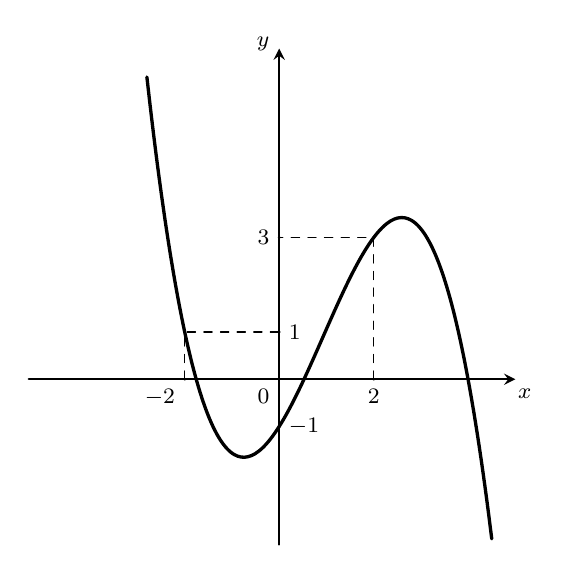
\begin{tikzpicture}[scale=0.6,font=\footnotesize, line join=round, line cap=round, >=stealth] %Đường cong bậc 3
			\draw[thick, ->] (-5.3,0)--(5,0);
			\draw[thick, ->] (0,-3.5)--(0,7);
			\draw (5.2,0) node[below] {$x$};
			\draw (0,7.1) node[left]{$y$};
			\draw (0,0) node[below left]{$0$};
			\draw[fill] (-2,0) circle (0.5pt)node[below left]{$ -2 $};
			\draw[fill] (2,0) circle (0.5pt)node[below]{$ 2$};
			\draw[fill] (0,3) circle (0.5pt)node[left]{$ 3 $};
			\draw[fill] (0,1) circle (0.5pt)node[right]{$ 1 $};
			\draw[fill] (0,-1) circle (0.5pt)node[right]{$ -1 $};
			\draw[dashed] (-2,0)--(-2,1) --(0,1); 
			\draw[dashed](2,0)--(2,3)--(0,3);
			\draw[line width=1.2pt,smooth,samples=100,domain=-2.8:4.5] plot(\x,{-0.271*(\x)^3+0.75*(\x)^2+1.583*\x-1});
		\end{tikzpicture}		
	}
	\loigiai{
		$\begin{aligned}
			& g(x)=4f\left(x^2\right)-x^6+5x^4-4x^2+1\Rightarrow g' (x)=8xf'\left(x^2\right)-6x^5+20x^3-8x.\\ 
			& g' (x)=0\Leftrightarrow 8xf'\left(x^2\right)-6x^5+20x^3-8x=0 \\
			& \Leftrightarrow 2x\left[4f'\left(x^2\right)-3x^4+10x^2-4\right]=0\\ 
			&\Leftrightarrow 		\hoac{ 			& 2x=0\\ 
				& 4f'(x^2)-3x^4+10x^2-4=0
			}
			\Leftrightarrow \hoac{	& x=0\\ 
				& f'\left(x^2\right)=\dfrac{3}{4}{x^4}-\dfrac{5}{2}{x^2}+1.}
		\end{aligned}$\\ 
		Xét
		$f'\left(x^2\right)=\dfrac{3}{4}x^4-\dfrac{5}{2}x^2+1$. Đặt $x^2=t+2$, ta có\\
		$ f' (t+2)=\dfrac{3}{4}{(t+2)^2}-\dfrac{5}{2}(t+2)+1=\dfrac{3}{4}\left(t^2+4t+4\right)-\dfrac{5}{2}(t+2)-1=\dfrac{3}{4}{t^2}+\dfrac{1}{2}t-1$\\
		Khi đó số nghiệm của phương trình chính là số giao điểm của đồ thị hàm số $y=f' (t+2)$ và\\
		$ y=\dfrac{3}{4}{t^2}+\dfrac{1}{2}t-1$\\
		Ta có đồ thị 
		\begin{center}
			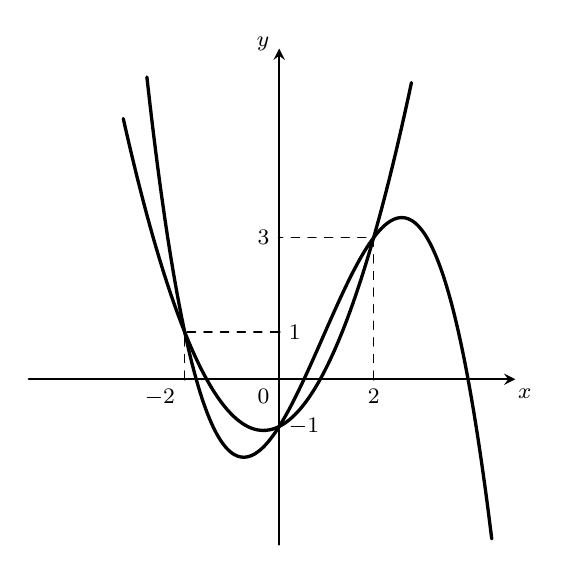
\begin{tikzpicture}[scale=0.6,font=\footnotesize, line join=round, line cap=round, >=stealth] %Đường cong bậc 3
				\draw[thick, ->] (-5.3,0)--(5,0);
				\draw[thick, ->] (0,-3.5)--(0,7);
				\draw (5.2,0) node[below] {$x$};
				\draw (0,7.1) node[left]{$y$};
				\draw (0,0) node[below left]{$0$};
				\draw[fill] (-2,0) circle (0.5pt)node[below left]{$ -2 $};
				\draw[fill] (2,0) circle (0.5pt)node[below]{$ 2$};
				\draw[fill] (0,3) circle (0.5pt)node[left]{$ 3 $};
				\draw[fill] (0,1) circle (0.5pt)node[right]{$ 1 $};
				\draw[fill] (0,-1) circle (0.5pt)node[right]{$ -1 $};
				\draw[dashed] (-2,0)--(-2,1) --(0,1); 
				\draw[dashed](2,0)--(2,3)--(0,3);
				\draw[line width=1.2pt,smooth,samples=100,domain=-2.8:4.5] plot(\x,{-0.271*(\x)^3+0.75*(\x)^2+1.583*\x-1});		
				\draw[line width=1.2pt,smooth,samples=100,domain=-3.3:2.8] plot(\x,{0.75*(\x)^2+0.5*\x-1});
			\end{tikzpicture}
		\end{center}
		Dựa vào đồ thị ta có $f' (t+2)=\dfrac{3}{4}t^2+\dfrac{1}{2}t-1\Leftrightarrow \hoac{& t=-2\\ & t=0\\ & t=2} \Leftrightarrow\hoac{& x+2=-2\\ & x+2=0\\ & x+2=2} \Leftrightarrow \hoac{& x=-4\\ & x=-2\\ & x=0.}$\\
		Ta có bảng xét dấu $g' (x)$ như sau
		\begin{center}
			
\begin{tikzpicture}
				\tkzTabInit[lgt=1.2,espcl=2,nocadre]
				{$x$/0.7, $f(x)$ /.7}
				{$-\infty$, $-4$,$-2$, $0$, $+\infty$} % first row
				\tkzTabLine { ,-,z,+,z,-,z,+, }
			\end{tikzpicture}
		\end{center}
		Vậy hàm số $g(x)=4 f\left(x^2\right)-x^6+5 x^4-4 x^2+1$ đồng biến trên khoảng $(2 ;+\infty)$.}
\end{ex}

\begin{ex}%[2D1G1-2]%Câu 30
	[Chuyên Bắc Ninh 2022] 
	\immini{
		Cho hàm số $ y=f(x)$ liên tục trên $\mathbb{R}$ có đồ thị hàm số $ y=f'(x)$ có đồ thị như hình vẽ bên.
		Hàm số $g(x)=2f\left(\left| x-1\right|\right)-x^2+2x+2020$ đồng biến trên khoảng nào
		\choice
		{$\left(-2;0\right)$}
		{$\left(-3;1\right)$}
		{$\left(1\,;3\right)$}
		{\True $\left(0\,;\,1\right)$}}{
		\begin{tikzpicture}[scale=0.6,font=\footnotesize, line join=round, line cap=round, >=stealth] %Đường cong bậc 3
			\draw[thick, ->] (-3.3,0)--(5,0);
			\draw[thick, ->] (0,-3.0)--(0,5.5);
			\draw (5.2,0) node[below] {$x$};
			\draw (0,5.8) node[left]{$y$};
			\draw (0,0) node[below left]{$0$};
			\draw[fill] (-1,0) circle (0.5pt)node[above]{$ -1 $};
			\draw[fill] (1,0) circle (0.5pt)node[below]{$ 1$};
			\draw[fill] (0,1) circle (0.5pt)node[left]{$ 1 $};
			\draw[fill] (0,-1) circle (0.5pt)node[right]{$ -1 $};
			\draw[fill] (0,3) circle (0.5pt)node[left]{$ 3 $};
			\draw[fill] (3,0) circle (0.5pt)node[below]{$ 3 $};
			\draw[dashed] (-1,0)--(-1,-1) --(0,-1); 
			\draw[dashed](1,0)--(1,1)--(0,1);
			\draw[dashed](3,0)--(3,3)--(0,3);
			\draw[line width=1.2pt,smooth,samples=100,domain=-2.2:4.3] plot(\x,{-0.333*(\x)^3+1*(\x)^2+1.333*\x-1});		
			%\draw[line width=1.2pt,smooth,samples=100,domain=-3.3:2.8] plot(\x,{0.75*(\x)^2+0.5*\x-1});
		\end{tikzpicture}	
	}
	\loigiai{
		Ta có $g(x)=2f\left(\left| x-1\right|\right)-x^2+2x+2020\Leftrightarrow g(x)=2f\left(\left| x-1\right|\right)-\left(x-1\right)^2+2021$.\\
		Xét hàm số $ k\left(x-1\right)=2f\left(x-1\right)-\left(x-1\right)^2+2021$.\\
		Đặt $ t=x-1$\\
		Xét hàm số $ h(t)=2f(t)-t^2+2021$ $\Rightarrow{h}'(t)=2f'(t)-2t$.\\
		Kẻ đường $ y=x$ như hình vẽ.
		\begin{center}
			\begin{tikzpicture}[scale=0.6,font=\footnotesize, line join=round, line cap=round, >=stealth] %Đường cong bậc 3
				\draw[thick, ->] (-3.3,0)--(5,0);
				\draw[thick, ->] (0,-3.0)--(0,5.5);
				\draw (5.2,0) node[below] {$x$};
				\draw (0,5.8) node[left]{$y$};
				%	\draw (0,0) node[below left]{$0$};
				\draw[fill] (-1,0) circle (0.5pt)node[above]{$ -1 $};
				\draw[fill] (1,0) circle (0.5pt)node[below]{$ 1$};
				\draw[fill] (0,1) circle (0.5pt)node[left]{$ 1 $};
				\draw[fill] (0,-1) circle (0.5pt)node[right]{$ -1 $};
				\draw[fill] (0,3) circle (0.5pt)node[left]{$ 3 $};
				\draw[fill] (3,0) circle (0.5pt)node[below]{$ 3 $};
				\draw[dashed] (-1,0)--(-1,-1) --(0,-1); 
				\draw[dashed](1,0)--(1,1)--(0,1);
				\draw[dashed](3,0)--(3,3)--(0,3);
				\draw[line width=1.2pt,smooth,samples=100,domain=-2.2:4.3] plot(\x,{-0.333*(\x)^3+1*(\x)^2+1.333*\x-1});		
				%\draw[line width=1.2pt,smooth,samples=100,domain=-3.3:2.8] plot(\x,{0.75*(\x)^2+0.5*\x-1});
				\draw[line width=1.2pt,smooth,samples=100](-2,-2)--(4,4);
			\end{tikzpicture}
		\end{center}
		Khi đó $h'(t)>0\Leftrightarrow{f}'(t)-t>0\Leftrightarrow{f}'(t)>t$$\Leftrightarrow \hoac{
			& t<-1\\ 
			& 1<t<3.
		}$\\
		Do đó $k'\left(x-1\right)>0\Leftrightarrow \hoac{
			& x-1<-1\\ 
			& 1<x-1<3} \Leftrightarrow \hoac{
			& x<0\\ 
			& 2<x<4.}$\\
		Ta có bảng biến thiên của hàm số $ k\left(x-1\right)=2f\left(x-1\right)-\left(x-1\right)^2+2021$.
		\begin{center}
			\begin{tikzpicture}
				\tkzTabInit[lgt=1.8,espcl=2.3]
				{$x$ /1.2, $k'(x-1)$ /1.2,$k(x-1)$ /2}
				{$-\infty$ , $0$,$2$,$4$, $+\infty$}
				\tkzTabLine{,+,0,-,0,+,0,-,}
				\tkzTabVar{-/$ $ ,+/$ $, -/$ $,+/$ $,-/$ $}
			\end{tikzpicture}
		\end{center}
		Khi đó, ta có bảng biến thiên của $g(x)=2f\left(\left| x-1\right|\right)-\left(x-1\right)^2+2021$ bằng cách lấy đối xứng qua đường thẳng $ x=1$ như sau\\
		\begin{center}
			\begin{tikzpicture}
				\tkzTabInit[lgt=1.2,espcl=2.5,nocadre]
				{$x$ /0.7, $g'(x)$ /0.7,$g(x)$ /2.5}
				{$-\infty$ ,$-2$, $0$,$1$,$2$,$4$, $+\infty$}
				\tkzTabLine{,+,0,-,0,+,0,-,0,+,0,-,}
				\tkzTabVar{-/$ $ ,+/$ $, -/$ $,+/$ $,-/$ $,+/ $ $,-/$ $}
			\end{tikzpicture}
		\end{center}
		Vậy hàm số đồng biến trên $\left(0;1\right)$.}
\end{ex}

\begin{ex}%[2D1G1-2]%Câu 31
	[Chuyên Thái Bình 2022] 
	\immini{
		Cho hàm số $f(x)=a{x^4}+b{x^3}+c{x^2}+dx+a$ có đồ thị hàm số $y=f'(x)$ như hình vẽ bên. Hàm số $y=g(x)=f\left(1-2x\right)f\left(2-x\right)$ đồng biến trên khoảng nào dưới đây?
		\choice
		{$\left(\dfrac{1}{2};\dfrac{3}{2}\right)$}
		{$\left(-\infty ;0\right)$}
		{$\left(0;2\right)$}
		{\True $\left(3;+\infty\right)$}}{
		\begin{tikzpicture}[scale=0.9,font=\footnotesize, line join=round, line cap=round, >=stealth] %Đường cong bậc 3
			\draw[thick, ->] (-2.5,0)--(2.5,0);
			\draw[thick, ->] (0,-2.8)--(0,2.8);
			\draw (2.6,0) node[below] {$x$};
			\draw (0,2.9) node[left]{$y$};
			\draw (0,0) node[below left]{$0$};
			\draw[fill] (-1,0) circle (0.5pt)node[below left]{$ -1 $};
			\draw[fill] (1,0) circle (0.5pt)node[below right]{$ 1$};
			%			\draw[dashed] (-1,0)--(-1,-1) --(0,-1); 
			%			\draw[dashed](1,0)--(1,1)--(0,1);
			%			\draw[dashed](3,0)--(3,3)--(0,3);
			\draw[line width=1.2pt,smooth,samples=100,domain=-1.3:1.3] plot(\x,{3*(\x)^3-3*\x});		
			%\draw[line width=1.2pt,smooth,samples=100,domain=-3.3:2.8] plot(\x,{0.75*(\x)^2+0.5*\x-1});
		\end{tikzpicture}	
	}
	\loigiai{
		Ta có $f'(x)=4a{x^3}+3b{x^2}+2cx+d$, theo đồ thị thì đa thức $f'(x)$ có ba nghiệm phân biệt là $-1,0,1$ nên $f'(x)=4ax\left(x+1\right)\left(x-1\right)=4a{x^3}-4ax\Rightarrow f(x)=a{x^4}-2a{x^2}+a=a{\left(x^2-1\right)^2}$.\\
		Dựa vào đồ thị hàm số $y=f'(x)$ ta có $a>0$ nên $f(x)>0,\forall x\in\mathbb{R}\setminus\left\{\pm 1\right\}$.\\
		$g'(x)=\left[f\left(1-2x\right)\right]'f\left(2-x\right)+f\left(1-2x\right)\left[f\left(2-x\right)\right]'=-2f'\left(1-2x\right)f\left(2-x\right)-f\left(1-2x\right)f'\left(2-x\right)$. Xét $x\in\left(\dfrac{1}{2};\dfrac{3}{2}\right)\Rightarrow
		\heva{		
			& 1-2x\in\left(-2;0\right)\\ 
			& 2-x\in\left(\dfrac{1}{2};\dfrac{3}{2}\right)}$, dấu của $f'(x)$ không cố định trên $\left(\dfrac{1}{2};\dfrac{3}{2}\right)$ nên ta không kết luận được tính đơn điệu của hàm số $g(x)$ trên $\left(\dfrac{1}{2};\dfrac{3}{2}\right)$.\\
		Xét $x\in\left(-\infty ;0\right)\Rightarrow
		\heva{
			& 1-2x\in\left(1;+\infty\right)\\ 
			& 2-x\in\left(2;+\infty\right)} 
		\Rightarrow \heva{
			& f'\left(1-2x\right)>0\\ 
			& f'\left(2-x\right)>0} \Rightarrow g'(x)<0$.\\
		Do đó, hàm số $g(x)$ nghịch biến trên $\left(-\infty ;0\right)$.\\
		$x\in\left(0;2\right)\Rightarrow \heva{
			& 1-2x\in\left(-3;1\right)\\ 
			& 2-x\in\left(0;2\right)}$, dấu của $f'(x)$ không cố định trên $\left(-3;1\right)$ và $\left(0;2\right)$ nên ta không kết luận được tính đơn điệu của hàm số $g(x)$ trên $\left(\dfrac{1}{2};\dfrac{3}{2}\right)$.\\
		Xét $x\in\left(3;+\infty\right)\Rightarrow \heva{
			& 1-2x\in\left(-\infty ;-5\right)\\ 
			& 2-x\in\left(-\infty ;-1\right)} \Rightarrow \heva{
			& f'\left(1-2x\right)<0\\ 
			& f'\left(2-x\right)<0} \Rightarrow g'(x)>0$. \\
		Do đó, hàm số $g(x)$ đồng biến trên $\left(3;+\infty\right)$.}
\end{ex}

\begin{dang}{Bài toán hàm ẩn, hàm hợp liên quan đến tham số và một số bài toán khác}
\end{dang}

\begin{ex}%[2D1G1-3]%Câu 1
	[Chuyên Lê Hồng Phong Nam Định 2019]
	\immini{
		Cho hàm số $ y=f(x)$ có đạo hàm liên tục trên $\mathbb{R}$. Biết hàm số $ y=f'(x)$ có đồ thị như hình vẽ. Gọi $ S$ là tập hợp các giá trị nguyên $ m\in\left[-5\,;\,\text{5}\right]$ để hàm số $ g(x)=f\left(x+m\right)$ nghịch biến trên khoảng $\left(1\,;\,2\right)$. Hỏi $S$ có bao nhiêu phần tử?
		\choice
		{$ 4$}
		{$ 3$}
		{$ 6$}
		{\True $ 5$}}{
		\begin{tikzpicture}[scale=0.9,font=\footnotesize, line join=round, line cap=round, >=stealth] %Đường cong bậc 3
			\draw[thick, ->] (-2.5,0)--(4,0);
			\draw[thick, ->] (0,-2.8)--(0,2.8);
			\draw (4.3,0) node[below] {$x$};
			\draw (0,2.9) node[left]{$y$};
			\draw (0,0) node[below left]{$0$};
			\draw[fill] (-1,0) circle (0.5pt)node[below left]{$ -1 $};
			\draw[fill] (1,0) circle (0.5pt)node[below]{$ 1$};
			\draw[fill] (3,0) circle (0.5pt)node[below right]{$ 3$};
			%			\draw[dashed] (-1,0)--(-1,-1) --(0,-1); 
			%			\draw[dashed](1,0)--(1,1)--(0,1);
			%			\draw[dashed](3,0)--(3,3)--(0,3);
			\draw[line width=1.2pt,smooth,samples=100,domain=-1.65:3.5] plot(\x,{0.33*(\x)^3-(\x)^2-0.333*(\x)+1});		
			%\draw[line width=1.2pt,smooth,samples=100,domain=-3.3:2.8] plot(\x,{0.75*(\x)^2+0.5*\x-1});
		\end{tikzpicture}	
	}
	\loigiai{
		Ta có $g'(x)=f'\left(x+m\right)$. Vì $ y=f'(x)$ liên tục trên $\mathbb{R}$ nên $g'(x)=f'\left(x+m\right)$ cũng liên tục trên $\mathbb{R}$. Căn cứ vào đồ thị hàm số $ y=f'(x)$ ta thấy\\
		$g'(x)<0\Leftrightarrow{f}'\left(x+m\right)<0$ $\Leftrightarrow\hoac{
			& x+m<-1\\ 
			& 1<x+m<3} \Leftrightarrow \hoac{
			& x<-1-m\\ 
			& 1-m<x<3-m.}$\\
		Hàm số $ g(x)=f\left(x+m\right)$ nghịch biến trên khoảng $\left(1\,;\,2\right)$
		$\Leftrightarrow \hoac{
			& 2\le-1-m\\ 
			&\hoac{
				& 3-m\ge 2\\ 
				& 1-m\le 1}} \Leftrightarrow \hoac{
			& m\le-3\\ 
			& 0\le m\le 1.}$\\
		Mà $ m$ là số nguyên thuộc đoạn $\left[-5\,;\,5\right]$ nên ta có $ S=\left\{-5;-4;-3;0;1\right\}$.\\
		Vậy $ S$ có $5$ phần tử.}
\end{ex}

\begin{ex}%[2D1G1-3]%Câu 2
	[Chuyên Nguyễn Bỉnh Khiêm-Quảng Nam-2020] Cho hàm số $ y=f(x)$ có đạo hàm trên $\mathbb{R}$ và bảng xét dấu đạo hàm như hình vẽ sau
	\begin{center}
		\begin{tikzpicture}
			\tkzTabInit[lgt=1.2,espcl=2.5,nocadre]
			{$x$/0.7, $f'(x)$ /2.5} % first column
			{$-\infty$, $-10$,$-2$, $3$,$8$, $+\infty$} % first row
			\tkzTabLine { ,+,z,-,z,+,z,-,z,+, } % second row
			%				\tkzTabLine {,-,z,+,t,+,} % third row
			%				\tkzTabLine {,+,d,-,z,+,} % last row
		\end{tikzpicture}
	\end{center}
	Có bao nhiêu số nguyên $ m$ để hàm số $ y=f\left(x^3+4x+m\right)$ nghịch biến trên khoảng $\left(-1;1\right)$?
	\choice
	{$ 3$}
	{$ 0$}
	{\True $ 1$}
	{$ 2$}
	\loigiai
	{
		Đặt $ t=x^3+4x+m\Rightarrow{t}'=3x^2+4$ nên $ t$ đồng biến trên $\left(-1;1\right)$ và $ t\in\left(m-5;m+5\right)$.\\
		Yêu cầu bài toán trở thành tìm $ m$ để hàm số $ f(t)$ nghịch biến trên khoảng $\left(m-5;m+5\right)$.\\
		Dựa vào bảng biến thiên ta được $\heva{
			& m-5\ge-2\\ 
			& m+5\le 8} \Leftrightarrow \heva{
			& m\ge 3\\ 
			& m\le 3} \Leftrightarrow m=3$.}
\end{ex}

\begin{ex}%[2D1G1-3]%Câu 3
	[Chuyên ĐH Vinh-Nghệ An-2020]
	\immini{
		Cho hàm số $ f(x)$ có đạo hàm trên $\mathbb{R}$và $ f(1)=1$. Đồ thị hàm số $ y=f'(x)$ như hình bên. Có bao nhiêu số nguyên dương $ a$ để hàm số $ y=\left| 4f\left(\sin x\right)+\cos 2x-a\right|$ nghịch biến trên $\left(0;\dfrac{\pi}{2}\right)$?
		\choice
		{$ 2$}
		{\True $ 3$}
		{Vô số}
		{$ 5$}}{
		\begin{tikzpicture}[scale=0.9,font=\footnotesize, line join=round, line cap=round, >=stealth] %Đường cong bậc 3
			\draw[thick, ->] (-2.5,0)--(3,0);
			\draw[thick, ->] (0,-2.8)--(0,2.8);
			\draw (3.1,0) node[below] {$x$};
			\draw (0,2.9) node[left]{$y$};
			\draw (0,0) node[below left]{$0$};
			\draw[fill] (-1,0) circle (0.5pt)node[below]{$ -1 $};
			\draw[fill] (1,0) circle (0.5pt)node[above]{$ 1$};
			%	\draw[fill] (3,0) circle (0.5pt)node[below right]{$ 3$};
			\draw[dashed] (-1,0)--(-1,1); 
			\draw[dashed](1,0)--(1,-1);
			%			\draw[dashed](3,0)--(3,3)--(0,3);
			\draw[line width=1.2pt,smooth,samples=100,domain=-2:2] plot(\x,{.8*(\x)^3+0*(\x)^2-1.8*(\x)});		
			%\draw[line width=1.2pt,smooth,samples=100,domain=-3.3:2.8] plot(\x,{0.75*(\x)^2+0.5*\x-1});
			\draw (2.0,2.8) node[left]{$y=f'(x)$};
		\end{tikzpicture}	
	}
	\loigiai
	{		Đặt $g(x)=\left| 4f\left(\sin x\right)+\cos 2x-a\right|\Rightarrow g(x)=\sqrt{\left[4f\left(\sin x\right)+\cos 2x-a\right]^2}$ .\\
		$\Rightarrow{g}'(x)=\dfrac{\left[4\cos x\cdot f'\left(\sin x\right)-2\sin 2x\right]\left[4f\left(\sin x\right)+\cos 2x-a\right]}{\sqrt{\left[4f\left(\sin x\right)+\cos 2x-a\right]^2}}$.\\
		Ta có $ 4\cos x\cdot f'\left(\sin x\right)-2\sin 2x=4\cos x\left[f'\left(\sin x\right)-\sin x\right]$.\\
		Với $ x\in\left(0;\dfrac{\pi}{2}\right)$ thì $\cos x>0,\sin x\in\left(0;1\right)\Rightarrow{f}'\left(\sin x\right)-\sin x<0$.\\
		Hàm số $ g(x)$ nghịch biến trên $\left(0;\dfrac{\pi}{2}\right)$ khi $ 4f\left(\sin x\right)+\cos 2x-a\ge 0,\forall x\in\left(0;\dfrac{\pi}{2}\right)$\\
		$\Leftrightarrow 4f\left(\sin x\right)+1-2\sin^2x\ge a,\forall x\in\left(0;\dfrac{\pi}{2}\right)$.\\
		Đặt $ t=\sin x$ được $ 4f(t)+1-2t^2\ge a,\forall t\in\left(0;1\right)$ (*).\\
		Xét $ h(t)=4f(t)+1-2t^2\Rightarrow{h}'(t)=4f'(t)-4t=4\left[f'(t)-1\right]$.\\
		Với $ t\in\left(0;1\right)$ thì $h'(t)<0\Rightarrow h(t)$ nghịch biến trên $\left(0;1\right)$.\\
		Do đó (*) $\Leftrightarrow a\le h(1)=4f(1)+1-2.1^2=3$.\\
		Vậy có $3$ giá trị nguyên dương của a thỏa mãn.}
\end{ex}


\begin{ex}%[2D1G1-3]%Câu 4
	[Chuyên Quang Trung-2020]
	\immini{
		Cho hàm số $ y=f(x)$ có đạo hàm liên tục trên $\mathbb{R}$ và có đồ thị $ y=f'(x)$ như hình vẽ. Đặt $ g(x)=f\left(x-m\right)-\dfrac{1}{2}{\left(x-m-1\right)^2}+2019$, với $ m$ là tham số thực. Gọi $ S$ là tập hợp các giá trị nguyên dương của $ m$ để hàm số $ y=g(x)$ đồng biến trên khoảng $\left(5;6\right)$. Tổng tất cả các phần tử trong $ S$ bằng
		\choice
		{$ 4$}
		{$ 11$}
		{\True $ 14$}
		{$ 20$}}{
		\begin{tikzpicture}[scale=0.9,font=\footnotesize, line join=round, line cap=round, >=stealth] %Đường cong bậc 3
			\draw[style=help lines,step=1] (-2.5,-3) grid (3,3.5);
			\draw[thick, ->] (-2.5,0)--(3.5,0);
			\draw[thick, ->] (0,-2.8)--(0,2.8);
			\draw (3.6,0) node[below] {$x$};
			\draw (0,3) node[above left]{$y$};
			\draw (0,0) node[below left]{$0$};
			%\draw[fill] (-1,0) circle (0.5pt)node[below]{$ -1 $};
			\draw[fill] (1,0) circle (0.5pt)node[below left]{$ 1$};
			%	\draw[fill] (3,0) circle (0.5pt)node[below right]{$ 3$};
			\draw[dashed] (-1,0)--(-1,-2) --(2,-2)--(2,0); 
			\draw[dashed](3,0)--(3,2) --(0,2);
			\draw (-1,-2) circle (2pt);
			\draw (3,2) circle (2pt);
			%			\draw[dashed](3,0)--(3,3)--(0,3);
			\draw[line width=1.2pt,smooth,samples=100,domain=-1.1:3.1] plot(\x,{1*(\x)^3-3*(\x)^2-0*(\x)+2});		
			%\draw[line width=1.2pt,smooth,samples=100,domain=-3.3:2.8] plot(\x,{0.75*(\x)^2+0.5*\x-1});
			%\draw (2.0,2.8) node[left]{$y=f'(x)$};
		\end{tikzpicture}	
	}
	\loigiai
	{
		Xét hàm số $ g(x)=f\left(x-m\right)-\dfrac{1}{2}{\left(x-m-1\right)^2}+2019$.\\
		$g'(x)=f'\left(x-m\right)-\left(x-m-1\right)$.\\
		Xét phương trình $g'(x)=0. \quad \quad (1)$\\
		Đặt $ x-m=t$, phương trình $(1)$ trở thành $f'(t)-\left(t-1\right)=0\Leftrightarrow{f}'(t)=t-1. \quad (2)$\\
		Nghiệm của phương trình $(2)$ là hoành độ giao điểm của hai đồ thị hàm số $ y=f'(t)$ và $ y=t-1$.\\
		Ta có đồ thị các hàm số $ y=f'(t)$ và $ y=t-1$ như sau
		\begin{center}
			\begin{tikzpicture}[scale=0.9,font=\footnotesize, line join=round, line cap=round, >=stealth] %Đường cong bậc 3
				\draw[style=help lines,step=1] (-2.5,-3) grid (3,3.5);
				\draw[thick, ->] (-2.5,0)--(3.5,0);
				\draw[thick, ->] (0,-2.8)--(0,2.8);
				\draw (3.6,0) node[below] {$x$};
				\draw (0,3) node[above left]{$y$};
				\draw (0,0) node[below left]{$0$};
				%\draw[fill] (-1,0) circle (0.5pt)node[below]{$ -1 $};
				\draw[fill] (1,0) circle (0.5pt)node[below left]{$ 1$};
				%	\draw[fill] (3,0) circle (0.5pt)node[below right]{$ 3$};
				\draw[dashed] (-1,0)--(-1,-2) --(2,-2)--(2,0); 
				\draw[dashed](3,0)--(3,2) --(0,2);
				\draw (-1,-2) circle (2pt);
				\draw (3,2) circle (2pt);
				%			\draw[dashed](3,0)--(3,3)--(0,3);
				\draw[line width=1.2pt,smooth,samples=100,domain=-1.1:3.1] plot(\x,{1*(\x)^3-3*(\x)^2-0*(\x)+2});		
				%\draw[line width=1.2pt,smooth,samples=100,domain=-3.3:2.8] plot(\x,{0.75*(\x)^2+0.5*\x-1});
				%\draw (2.0,2.8) node[left]{$y=f'(x)$};
				\draw (-2,-3)--(4,3);
			\end{tikzpicture}
		\end{center}
		Căn cứ đồ thị các hàm số ta có phương trình $(2)$ có nghiệm là $\hoac{
			& t=-1\\ 
			& t=1\\ 
			& t=3} \Rightarrow \hoac{
			& x=m-1\\ 
			& x=m+1\\ 
			& x=m+3.}$\\
		Ta có bảng biến thiên của $ y=g(x)$
		\begin{center}
			\begin{tikzpicture}
				\tkzTabInit[lgt=1,espcl=2.5,nocadre]
				{$x$ /0.8, $y'$ /0.8,$y$ /2.5}
				{$-\infty$ , $m-1$,$m+1$,$m+3$, $+\infty$}
				\tkzTabLine{,+,0,-,0,+,0,-,}
				\tkzTabVar{-/$ +\infty$ ,+/$ $, -/$ $,+/$ $,-/$+\infty $}
			\end{tikzpicture}
		\end{center}
		Để hàm số $ y=g(x)$ đồng biến trên khoảng $\left(5;6\right)$ cần $\hoac{
			&\heva{
				& m-1\le 5\\ 
				& m+1\ge 6}\\ 
			& m+3\le 5}\Leftrightarrow\hoac{
			& 5\le m\le 6\\ 
			& m\le 2.}$\\
		Vì $ m\in\mathbb{N}^*\Rightarrow m$ nhận các giá trị $ 1;\,2;\,5;\,6\Rightarrow S=14$.}
\end{ex}

\begin{ex}%[2D1G1-3]%Câu 5
	[Sở Hà Nội-Lần 2-2020] 
	\immini{
		Cho hàm số $y=a{x^4}+b{x^3}+c{x^2}+dx+e,\,\,a\ne 0$. Hàm số $y=f'(x)$ có đồ thị như hình vẽ bên. 
		Gọi S là tập hợp tất cả các giá trị nguyên thuộc khoảng $\left(-6;6\right)$ của tham số $m$ để hàm số $g(x)=f\left(3-2x+m\right)+x^2-\left(m+3\right)x+2m^2$ nghịch biến trên $\left(0;1\right)$. Khi đó, tổng giá trị các phần tử của S là
		\choice
		{$12$}
		{\True $9$}
		{$6$}
		{$15$}}{
		\begin{tikzpicture}[scale=0.7,font=\footnotesize, line join=round, line cap=round, >=stealth] %Đường cong bậc 3
			%	\draw[style=help lines,step=1] (-2.5,-3) grid (3,3.5);
			\draw[thick, ->] (-4.5,0)--(6.5,0);
			\draw[thick, ->] (0,-2.8)--(0,2.8);
			\draw (6.6,0) node[below] {$x$};
			\draw (0,3) node[above left]{$y$};
			\draw (0,0) node[below left]{$0$};
			\draw[fill] (-2,0) circle (0.5pt)node[below]{$ -2 $};
			\draw[fill] (4,0) circle (0.5pt)node[above]{$ 4$};
			\draw[fill] (0,1) circle (0.5pt)node[right]{$ 1 $};
			\draw[fill] (0,-2) circle (0.5pt)node[left]{$ -2$};
			%	\draw[fill] (3,0) circle (0.5pt)node[below right]{$ 3$};
			\draw[dashed] (-2,0)--(-2,1) --(0,1); 
			\draw[dashed](4,0)--(4,-2) --(0,-2);
			%			\draw[dashed](3,0)--(3,3)--(0,3);
			\draw[line width=1.2pt,smooth,samples=100,domain=-3.8:5.5] plot(\x,{0.0714*(\x)^3-0.1423*(\x)^2-1.0714*(\x)});		
			%\draw[line width=1.2pt,smooth,samples=100,domain=-3.3:2.8] plot(\x,{0.75*(\x)^2+0.5*\x-1});
			%\draw (2.0,2.8) node[left]{$y=f'(x)$};
		\end{tikzpicture}	
	}
	\loigiai
	{
		Xét $g'(x)=-2f'\left(3-2x+m\right)+2x-\left(m+3\right)$.\\
		Xét phương trình $g'(x)=0$, đặt $t=3-2x+m$ thì phương trình trở thành\\ $-2\cdot \left[f'(t)-\dfrac{-t}{2}\right]=0\Leftrightarrow\hoac{
			& t=-2\\ 
			& t=4\\ 
			& t=0.}$ \\
		Từ đó, $g'(x)=0\Leftrightarrow{x_1}=\dfrac{5+m}{2},\,x_2=\dfrac{m+3}{2},x_3=\dfrac{-1+m}{2}$.\\
		Lập bảng xét dấu, đồng thời lưu ý nếu $x>x_1$ thì $t<t_1$ nên $f(x)>0$. Và các dấu đan xen nhau do các nghiệm đều làm đổi dấu đạo hàm nên suy ra $g'(x)\le 0\Leftrightarrow x\in\left[x_2;{x_1}\right]\cup\left(-\infty ;{x_3}\right]$.\\
		Vì hàm số nghịch biến trên $\left(0;1\right)$ nên \\
		$g'(x)\le 0,\,\forall x\in\left(0;1\right)$ từ đó suy ra $\hoac{
			&\dfrac{3+m}{2}\le 0<1\le\dfrac{5+m}{2}\\ 
			& 1\le\dfrac{-1+m}{2}.}$ \\
		và giải ra các giá trị nguyên thuộc $\left(-6;6\right)$ của $m$ là $-3$; $3$; $4$; $5$. }
\end{ex}

\begin{ex}%[2D1G1-3]%Câu 6
	[Chuyên Quang Trung-Bình Phước-Lần 2-2020]
	\immini{
		Cho hàm số $ y=f(x)$ có đạo hàm liên tục trên $\mathbb{R}$ và có đồ thị $ y=f'(x)$ như hình vẽ bên. Đặt $ g(x)=f\left(x-m\right)-\dfrac{1}{2}{\left(x-m-1\right)^2}+2019$, với $ m$ là tham số thực. Gọi $ S$ là tập hợp các giá trị nguyên dương của $ m$ để hàm số $ y=g(x)$ đồng biến trên khoảng $\left(5;6\right)$. Tổng tất cả các phần tử trong $ S$ bằng
		\choice
		{$ 4$}
		{$ 11$}
		{\True $ 14$}
		{$ 20$}}{
		\begin{tikzpicture}[scale=0.9,font=\footnotesize, line join=round, line cap=round, >=stealth] %Đường cong bậc 3
			\draw[thick, ->] (-2.5,0)--(3.7,0);
			\draw[thick, ->] (0,-2.8)--(0,2.8);
			\draw (3.9,0) node[below] {$x$};
			\draw (0,2.9) node[left]{$y$};
			\draw (0,0) node[below left]{$0$};
			\draw[fill] (-1,0) circle (0.5pt)node[above]{$ -1 $};
			\draw[fill] (1,0) circle (0.5pt)node[below]{$ 1$};
			\draw[fill] (3,0) circle (0.5pt)node[below]{$ 3$};
			\draw[fill] (2,0) circle (0.5pt)node[above]{$ 2$};
			\draw[fill] (0,2) circle (0.5pt)node[above left]{$ 2$};
			\draw[fill] (0,-2) circle (0.5pt)node[below left]{$ -2$};
			\draw[dashed] (-1,0)--(-1,-2)--(2,-2)--(2,0); 
			\draw[dashed](3,0)--(3,2)--(0,2);
			%			\draw[dashed](3,0)--(3,3)--(0,3);
			\draw[line width=1.2pt,smooth,samples=100,domain=-1.1:3.1] plot(\x,{1*(\x)^3-3*(\x)^2-0*(\x)+2});		
			%\draw[line width=1.2pt,smooth,samples=100,domain=-3.3:2.8] plot(\x,{0.75*(\x)^2+0.5*\x-1});
			%	\draw (2.0,2.8) node[left]{$y=f'(x)$};
	\end{tikzpicture}	}
	\loigiai
	{
		Ta có $g'(x)=f'\left(x-m\right)-\left(x-m-1\right)$.\\
		Cho $g'(x)=0\Leftrightarrow{f}'\left(x-m\right)=x-m-1$.\\
		Đặt $ x-m=t\Rightarrow f'(t)=t-1$\\
		Khi đó nghiệm của phương trình là hoành độ giao điểm của đồ thị hàm số $ y=f'(t)$ và và đường thẳng $ y=t-1$.
		\begin{center}
			\begin{tikzpicture}[scale=0.9,font=\footnotesize, line join=round, line cap=round, >=stealth] %Đường cong bậc 3
				\draw[thick, ->] (-2.5,0)--(3.7,0);
				\draw[thick, ->] (0,-2.8)--(0,2.8);
				\draw (3.9,0) node[below] {$x$};
				\draw (0,2.9) node[left]{$y$};
				\draw (0,0) node[below left]{$0$};
				\draw[fill] (-1,0) circle (0.5pt)node[above]{$ -1 $};
				\draw[fill] (1,0) circle (0.5pt)node[below]{$ 1$};
				\draw[fill] (3,0) circle (0.5pt)node[below]{$ 3$};
				\draw[fill] (2,0) circle (0.5pt)node[above]{$ 2$};
				\draw[fill] (0,2) circle (0.5pt)node[above left]{$ 2$};
				\draw[fill] (0,-2) circle (0.5pt)node[below left]{$ -2$};
				\draw[dashed] (-1,0)--(-1,-2)--(2,-2)--(2,0); 
				\draw[dashed](3,0)--(3,2)--(0,2);
				%			\draw[dashed](3,0)--(3,3)--(0,3);
				\draw[line width=1.2pt,smooth,samples=100,domain=-1.1:3.1] plot(\x,{1*(\x)^3-3*(\x)^2-0*(\x)+2});		
				%\draw[line width=1.2pt,smooth,samples=100,domain=-3.3:2.8] plot(\x,{0.75*(\x)^2+0.5*\x-1});
				%	\draw (2.0,2.8) node[left]{$y=f'(x)$};
				\coordinate (a) at ($(-1,-2)!1.2!(3,2)$);
				\coordinate (b) at ($(-1,-2)!-.2!(3,2)$);
				\draw[line width=1.2pt,smooth] (a)--(b);
			\end{tikzpicture}
		\end{center}
		Dựa vào đồ thị hàm số ta có được $f'(t)=t-1\Leftrightarrow\hoac{
			& t=-1\\ 
			& t=1\\ 
			& t=3.} $ \\
		Bảng xét dấu của $g'(t)$
		\begin{center}
			\begin{tikzpicture}
				\tkzTabInit[lgt=1.2,espcl=2.5,nocadre]
				{$t$/1, $g'(x)$ /.8} % first column
				{$-\infty$, $-1$,$1$, $3$, $+\infty$} % first row
				\tkzTabLine { ,-,0,+,0,-,0,+, } % second row
				%				\tkzTabLine {,-,z,+,t,+,} % third row
				%				\tkzTabLine {,+,d,-,z,+,} % last row
			\end{tikzpicture}
		\end{center}
		Từ bảng xét dấu ta thấy hàm số $ g(t)$ đồng biến trên khoảng $\left(-1;1\right)$ và $\left(3;+\infty\right)$.\\
		Hay $\hoac{
			&-1<t<1\\ 
			& t>3}\Leftrightarrow\hoac{
			&-1<x-m<1\\ 
			& x-m>3} \Leftrightarrow\hoac{
			& m-1<x<m+1\\ 
			& x>m+3.}$\\
		Để hàm số $ g(x)$ đồng biến trên khoảng $\left(5;6\right)$ thì $\hoac{
			& m-1\le 5<6\le m+1\\ 
			& m+3\le 5<6} \Leftrightarrow\hoac{
			& 5\le m\le 6\\ 
			& m\le 2.}$\\
		Vì $ m$ là các số nguyên dương nên $ S=\left\{ 1;2;5;6\right\}$.\\
		Vậy tổng tất cả các phần tử của $ S$ là $ 1+2+5+6=14$.}
\end{ex}

\begin{ex}%[2D1G1-3]%Câu 7
	\immini{
		Cho hàm số $ y=f(x)$ liên tục có đạo hàm trên $\mathbb{R}$. Biết hàm số $ f'(x)$ có đồ thị cho như hình vẽ bên. Có bao nhiêu giá trị nguyên của $ m$ thuộc $\left[-2019;2019\right]$ để hàm só $ g(x)=f\left(2019^x\right)-mx+2$ đồng biến trên $\left[0;1\right]$.
		\choice
		{$ 2028$}
		{$ 2019$}
		{$ 2011$}
		{\True $ 2020$}}{
		\begin{tikzpicture}[scale=0.9,font=\footnotesize, line join=round, line cap=round, >=stealth] %Đường cong bậc 3
			\draw[thick, ->] (-3.5,0)--(2.5,0);
			\draw[thick, ->] (0,-2.8)--(0,2.8);
			\draw (2.7,0) node[below] {$x$};
			\draw (0,2.9) node[left]{$y$};
			\draw (0,0) node[below left]{$0$};
			%	\draw[fill] (-1,0) circle (0.5pt)node[above]{$ -1 $};
			\draw[fill] (1,0) circle (0.5pt)node[below right]{$ 1$};
			%		\draw[fill] (3,0) circle (0.5pt)node[below]{$ 3$};
			%		\draw[fill] (2,0) circle (0.5pt)node[above]{$ 2$};
			%		\draw[fill] (0,2) circle (0.5pt)node[above left]{$ 2$};
			%		\draw[fill] (0,-2) circle (0.5pt)node[below left]{$ -2$};
			%		\draw[dashed] (-1,0)--(-1,-2)--(2,-2)--(2,0); 
			%		\draw[dashed](3,0)--(3,2)--(0,2);
			\draw[line width=1.2pt,smooth,samples=100,domain=-3.28:1.32] plot(\x,{0.667*(\x)^3+2*(\x)^2-0.667*(\x)-2});		
			%\draw[line width=1.2pt,smooth,samples=100,domain=-3.3:2.8] plot(\x,{0.75*(\x)^2+0.5*\x-1});
			%	\draw (2.0,2.8) node[left]{$y=f'(x)$};
	\end{tikzpicture}	}
	\loigiai{
		Ta có $ g'(x)=2019^x\ln 2019\cdot f'\left(2019^x\right)-m$.\\
		Ta lại có hàm số $ y=2019^x$ đồng biến trên $\left[0;1\right]$.\\
		Với $ x\in\left[0;1\right]$ thì $2019^x\in\left[1;2019\right]$ mà hàm $ y=f'(x)$ đồng biến trên $\left(1;+\infty\right)$ nên hàm $ y=f'\left(2019^x\right)$ đồng biến trên $\left[0;1\right]$.\\
		Mà $2019^x\ge 1;f'\left(2019^x\right)>0\,\forall\,x\in\left[0;1\right]$ nên hàm $ h(x)=2019^x\ln 2019\cdot f'\left(2019^x\right)$ đồng biến trên $\left[0;1\right]$.\\
		Hay $ h(x)\ge h(0)=0,\forall\,x\in\left[0;1\right]$.\\
		Do vậy hàm số $ g(x)$ đồng biến trên đoạn $\left[0;1\right]$$\Leftrightarrow g'(x)\ge 0,\forall\,x\in\left[0;1\right]$\\
		$\Leftrightarrow m\le{2019^x}\ln 2019.f'\left(2019^x\right),\forall\,x\in\left[0;1\right]$ $\Leftrightarrow m\le\underset{x\in\left[0;1\right]}{\min}\,h(x)=h(0)=0$\\
		Vì $ m$ nguyên và $ m\in\left[-2019;2019\right]\Rightarrow $có $ 2020$ giá trị $ m$ thỏa mãn yêu cầu bài toán.}
\end{ex}

\begin{ex}%[2D1G1-3]%Câu 8
	\immini{
		Cho hàm số $y=f(x)$ có đồ thị $f'(x)\,$ như hình vẽ. Có bao nhiêu giá trị nguyên $m\in\left(-2020\,;\,2020\right)$ để hàm số $g(x)=f\left(2x-3\right)\,-\ln \left(1+x^2\right)-2mx$ đồng biến trên $\left(\dfrac{1}{2};2\right)$?
		\choice
		{$ 2020$}
		{\True $ 2019$}
		{$ 2021$}
		{$ 2018$}}{
		\begin{tikzpicture}[scale=0.9,font=\footnotesize, line join=round, line cap=round, >=stealth] %Đường cong bậc 3
			\draw[thick, ->] (-2.5,0)--(2.5,0);
			\draw[thick, ->] (0,-1.8)--(0,5.8);
			\draw (2.7,0) node[below] {$x$};
			\draw (0,5.9) node[left]{$y$};
			\draw (0,0) node[below left]{$0$};
			\draw[fill] (-2,0) circle (0.5pt)node[below]{$ -2 $};
			\draw[fill] (1,0) circle (0.5pt)node[below]{$ 1$};
			\draw[fill] (-1,0) circle (0.5pt)node[below]{$-1$};
			\draw[fill] (0,4) circle (0.5pt)node[above left]{$ 2$};
			%		\draw[fill] (0,2) circle (0.5pt)node[above left]{$ 2$};
			%		\draw[fill] (0,-2) circle (0.5pt)node[below left]{$ -2$};
			\draw[dashed] (-2,0)--(-2,4)--(1,4)--(1,0); 
			%		\draw[dashed](3,0)--(3,2)--(0,2);
			\draw[line width=1.2pt,smooth,samples=100,domain=-2.1:2.1] plot(\x,{-1*(\x)^3+0*(\x)^2+3*(\x)+2});		
			%\draw[line width=1.2pt,smooth,samples=100,domain=-3.3:2.8] plot(\x,{0.75*(\x)^2+0.5*\x-1});
			%	\draw (2.0,2.8) node[left]{$y=f'(x)$};
	\end{tikzpicture}	}
	\loigiai{
		Ta có $g'(x)=2f'\left(2x-3\right)-\dfrac{2x}{1+x^2}-2m$.\\
		Hàm số $ g(x)$ đồng biến trên $\left(\dfrac{1}{2};2\right)$ khi và chỉ khi \\
		$g'(x)\ge 0,\,\,\forall x\in\left(-1;\,2\right)$\\
		$\Leftrightarrow m\le{f}'\left(2x-3\right)-\dfrac{x}{1+x^2},\,\,\forall x\in\left(\dfrac{1}{2};2\right)$\\
		$\Leftrightarrow m\le\underset{x\in\left[\dfrac{1}{2};2\right]}{\min}\,\left[f'\left(2x-3\right)-\dfrac{x}{1+x^2}\right]$. \, \,  $(1)$\\
		Đặt $ t=2x-3$, khi đó $ x\in\left(\dfrac{1}{2};2\right)\Leftrightarrow t\in\left(-2;\,1\right)$.\\
		Từ đồ thị hàm $f'(x)$ suy ra $f'(t)\ge 0,\,\,\forall t\in\left(-2;1\right)$ và $f'(t)=0$ khi $ t=-1$.\\
		Tức là $f'\left(2x-3\right)\ge 0,\,\,\forall x\in\left(\dfrac{1}{2};\,2\right)$$\Rightarrow\underset{x\in\left[\dfrac{1}{2};2\right]}{\min}\,f'\left(2x-3\right)=0$ khi $ x=1$. $(2)$\\
		Xét hàm số $ h(x)=-\dfrac{x}{1+x^2}$ trên khoảng $\left(\dfrac{1}{2};\,2\right)$.\\
		Ta có $h'(x)=\dfrac{x^2-1}{\left(1+x^2\right)^2}$ và\\
		$h'(x)=0\Leftrightarrow{x^2}-1=0\Leftrightarrow x=\pm 1$.\\
		Bảng biến thiên của hàm số $ h(x)$ trên $\left(\dfrac{1}{2};\,2\right)$ như sau
		\begin{center}
			\begin{tikzpicture}
				\tkzTabInit[lgt=1.2,espcl=2.5,nocadre]
				{$x$ /0.7, $h'(x)$ /0.7,$h(x)$ /2.5}
				{$\dfrac{1}{2}$ , $1$,$2$}
				\tkzTabLine{,-,0,+,}
				\tkzTabVar{+/$  $ ,-/$ \-\dfrac{1}{2} $, +/$ $}
			\end{tikzpicture}
		\end{center}
		Từ bảng biến thiên suy ra $ h(x)\ge-\dfrac{1}{2}$$\Rightarrow\underset{x\in\left[\dfrac{1}{2};2\right]}{\min}\,h(x)=-\dfrac{1}{2}$ khi $ x=1$. \, \,  $(3)$\\
		Từ $(1)$, $(2)$ và $(3)$ suy ra $ m\le-\dfrac{1}{2}$.\\
		Kết hợp với $ m\in\mathbb{Z}$, $ m\in\left(-2020;\,2020\right)$ thì $ m\in\left\{-2019;\,-201;\ldots ;-2;-1\right\}$.\\
		Vậy có tất cả $ 2019$ giá trị $ m$ cần tìm.}
\end{ex}

\begin{ex}%[2D1G1-3]%Câu 9
	Cho hàm số $ f(x)$ liên tục trên $\mathbb{R}$ và có đạo hàm $f'(x)=x^2\left(x-2\right)\left(x^2-6x+m\right)$ với mọi $ x\in\mathbb{R}$. Có bao nhiêu số nguyên $ m$ thuộc đoạn $\left[-2020;2020\right]$ để hàm số $ g(x)=f\left(1-x\right)$ nghịch biến trên khoảng $\left(-\infty ;-1\right)$?
	\choice
	{$ 2016$}
	{$ 2014$}
	{\True $ 2012$}
	{$ 2010$}
	\loigiai{
		Ta có \\
		$g'(x)=f'\left(1-x\right)=-\left(1-x\right)^2\left(-x-1\right)\left[\left(1-x\right)^2-6\left(1-x\right)+m\right]$
		$=\left(x-1\right)^2\left(x+1\right)\left(x^2+4x+m-5\right)$.\\
		Hàm số $ g(x)$ nghịch biến trên khoảng $\left(-\infty ;-1\right)$\\
		$\Leftrightarrow{g}'(x)\le 0,\forall x<-1$ $(*)$, (dấu \lq\lq $=$\rq\rq \, xảy ra tại hữu hạn điểm).\\
		Với $ x<-1$ thì $\left(x-1\right)^2>0$ và $ x+1<0$ nên\\
		$(*)$ $\Leftrightarrow{x^2}+4x+m-5\ge 0,\forall x<-1 \Leftrightarrow m\ge-x^2-4x+5,\forall x<-1$.\\
		Xét hàm số $ y=-x^2-4x+5$ trên khoảng $\left(-\infty ;-1\right)$, ta có bảng biến thiên
		\begin{center}
			\begin{tikzpicture}
				\tkzTabInit[lgt=1.8,espcl=2.3]
				{$x$ /1.2, $y'$ /1.2,$y$ /2}
				{$-\infty$ , $-2$,$-1$}
				\tkzTabLine{,+,0,-,}
				\tkzTabVar{-/$ -\infty $ ,+/$9 $, -/$ 8$}
			\end{tikzpicture}
		\end{center}
		Từ bảng biến thiên suy ra $ m\ge 9$.\\
		Kết hợp với $ m$ thuộc đoạn $\left[-2020;2020\right]$ và $ m$ nguyên nên $ m\in\left\{ 9;10;11;\ldots ;2020\right\}$.\\
		Vậy có $ 2012$ số nguyên $ m$ thỏa mãn đề bài.}
\end{ex}

\begin{ex}%[2D1G1-3]%Câu 10
	\immini{
		Cho hàm số $f(x)$ xác định và liên tục trên $ R$. Hàm số $y=f'(x)$ liên tục trên $\mathbb{R}$ và có đồ thị như hình vẽ bên.
		Xét hàm số $g(x)=f\left(x-2m\right)+\dfrac{1}{2}{\left(2m-x\right)^2}+2020$, với $ m$ là tham số thực. Gọi $ S$ là tập hợp các giá trị nguyên dương của $ m$ để hàm số $ y=g(x)$ nghịch biến trên khoảng $\left(3;4\right)$. Hỏi số phần tử của $ S$ bằng bao nhiêu?
		\choice
		{$4$}
		{\True $2$}
		{$3$}
		{Vô số}}
	{
		\begin{tikzpicture}[scale=0.7,>=stealth, font=\footnotesize, line join=round, line cap=round]
			\def\xmin{-3.5} \def\xmax{4.5}
			\def\ymin{-5.2} \def\ymax{4}
			\clip(\xmin,\ymin) rectangle (\xmax,\ymax);
			\draw[->] (\xmin,0)--(\xmax,0) node [below]{$x$};
			\draw[->] (0,\ymin)--(0,\ymax) node [left]{$y$};
			\node at (0,0) [below left]{$O$};
			\path
			(-3.1,3.7) coordinate (A)
			(-3,3) coordinate (B)
			(0,-2) coordinate (C)
			(0.65,-2) coordinate (D)
			(1,-1) coordinate (E)
			(3,-3) coordinate (F)
			(3.4,-5) coordinate (G);
			\draw[smooth]
			(A)..controls +(-88:0.1) and +(93:.1)..
			(B)..controls +(-87:0.3) and +(-100:8.5)..
			(C)..controls +(75:.8) and +(180:.1)..
			(D)..controls +(0:.1) and +(-105:.3)..
			(E)..controls +(70:2) and +(97:0.4)..
			(F)..controls +(-80:.1) and +(90:0.3)..
			(G);
			\draw[dashed] 
			(-3,0)node[below]{$-3$}|-(0,3)node[right]{$3$}
			(1,0)node[above]{$1$}|-(0,-1)node[left]{$-1$}
			(3,0)node[above]{$3$}|-(0,-3)node[below right]{$-3$};
			\fill 
			(0,-2) circle(1.5pt)
			(-3,3) circle(1.5pt)
			(3,-3) circle(1.5pt)
			(1,-1) circle(1.5pt);
			\node at (2.1,-4) {$y=f'(x)$};
		\end{tikzpicture}
	}
	\loigiai{
		Ta có $g'(x)=f'\left(x-2m\right)-\left(2m-x\right)$.		Đặt $h(x)=f'(x)-\left(-x\right)$.\\
		Từ đồ thị hàm số $y=f'(x)$ và đồ thị hàm số $y=-x$ trên hình vẽ suy ra \\
		$h(x)\le 0\Leftrightarrow f'(x)\le-x\Leftrightarrow\hoac{
			&-3\le x\le 1\\ 
			& x\ge 3.}$ 
		\begin{center}
			\begin{tikzpicture}[scale=0.7,>=stealth, font=\footnotesize, line join=round, line cap=round]
				\def\xmin{-3.5} \def\xmax{4.5}
				\def\ymin{-5.2} \def\ymax{4}
				\clip(\xmin,\ymin) rectangle (\xmax,\ymax);
				\draw[->] (\xmin,0)--(\xmax,0) node [below]{$x$};
				\draw[->] (0,\ymin)--(0,\ymax) node [left]{$y$};
				\node at (0,0) [below left]{$O$};
				\path
				(-3.1,3.7) coordinate (A)
				(-3,3) coordinate (B)
				(0,-2) coordinate (C)
				(0.65,-2) coordinate (D)
				(1,-1) coordinate (E)
				(3,-3) coordinate (F)
				(3.4,-5) coordinate (G);
				\draw[smooth]
				(A)..controls +(-88:0.1) and +(93:.1)..
				(B)..controls +(-87:0.3) and +(-100:8.5)..
				(C)..controls +(75:.8) and +(180:.1)..
				(D)..controls +(0:.1) and +(-105:.3)..
				(E)..controls +(70:2) and +(97:0.4)..
				(F)..controls +(-80:.1) and +(90:0.3)..
				(G);
				\draw[dashed] 
				(-3,0)node[below]{$-3$}|-(0,3)node[right]{$3$}
				(1,0)node[above]{$1$}|-(0,-1)node[left]{$-1$}
				(3,0)node[above]{$3$}|-(0,-3)node[below right]{$-3$};
				\fill 
				(0,-2) circle(1.5pt)
				(-3,3) circle(1.5pt)
				(3,-3) circle(1.5pt)
				(1,-1) circle(1.5pt);
				\draw[smooth,samples=300,domain=-3.2:3.7] plot(\x,{-(\x)});
				\node at (2.1,-4) {$y=f'(x)$};
				\node at (-1,2.1) {$y=h(x)$};
			\end{tikzpicture}
		\end{center}
		Ta có $ g'(x)=h\left(x-2m\right)\le 0\Leftrightarrow\hoac{
			&-3\le x-2m\le 1\\ 
			& x-2m\ge 3}\Leftrightarrow\hoac{
			& 2m-3\le x\le 2m+1\\ 
			& x\ge 2m+3.}$.\\
		Suy ra hàm số $ y=g(x)$ nghịch biến trên các khoảng $\left(2m-3;2m+1\right)$ và $\left(2m+3;+\infty\right)$.\\
		Do đó hàm số $ y=g(x)$ nghịch biến trên khoảng $\left(3;4\right)$ $\Leftrightarrow\hoac{
			&\heva{
				& 2m-3\le 3\\ 
				& 2m+1\ge 4}\\ 
			& 2m+3\le 3}\Leftrightarrow\hoac{
			&\dfrac{3}{2}\le m\le 3\\ 
			& m\le 0.}$ \\
		Mặt khác, do $ m$ nguyên dương nên $ m\in\left\{ 2;3\right\}\Rightarrow S=\left\{ 2;3\right\}$. Vậy số phần tử của $ S$ bằng $2$.\\
	}
	
\end{ex}

\begin{ex}%[2D1G1-3]%Câu 11
	Cho hàm số $f(x)$ có đạo hàm trên $\mathbb{R}$ là $f'(x)=\left(x-1\right)\left(x+3\right)$. Có bao nhiêu giá trị nguyên của tham số $m$ thuộc đoạn $\left[-10;20\right]$ để hàm số $y=f\left(x^2+3x-m\right)$ đồng biến trên khoảng $\left(0;2\right)$?
	\choice
	{\True $ 18$}
	{$ 17$}
	{$ 16$}
	{$ 20$}
	\loigiai{
		Ta có $y'=f'\left(x^2+3x-m\right)=\left(2x+3\right){f}'\left(x^2+3x-m\right)$.\\
		Theo đề bài ta có $f'(x)=\left(x-1\right)\left(x+3\right)$\\
		suy ra $f'(x)>0\Leftrightarrow\hoac{
			& x<-3\\ 
			& x>1}$ và $f'(x)<0\Leftrightarrow-3<x<1$ .\\
		Hàm số đồng biến trên khoảng $\left(0;2\right)$ khi $y'\ge 0,\forall x\in\left(0;2\right)$\\
		$\Leftrightarrow\left(2x+3\right){f}'\left(x^2+3x-m\right)\ge 0,\forall x\in\left(0;2\right)$.\\
		Do $x\in\left(0;2\right)$ nên $2x+3>0,\forall x\in\left(0;2\right)$. Do đó, ta có\\
		$y'\ge 0,\forall x\in\left(0;2\right)\Leftrightarrow f'\left(x^2+3x-m\right)\ge 0$\\
		$\Leftrightarrow\hoac{
			&{x^2}+3x-m\le-3\\ 
			&{x^2}+3x-m\ge 1}\Leftrightarrow\hoac{
			& m\ge{x^2}+3x+3\\ 
			& m\le{x^2}+3x-1}$\\
		$\Leftrightarrow\hoac{
			& m\ge\underset{\left[0;2\right]}{\max}\,\left(x^2+3x+3\right)\\ 
			& m\le\underset{\left[0;2\right]}{\min}\,\left(x^2+3x-1\right)} \Leftrightarrow\hoac{
			& m\ge 13\\ 
			& m\le-1}$.\\
		Do $m\in\left[-10;20\right]$, $ m\in\mathbb{Z}$ nên có $ 18$ giá trị nguyên của $m$ thỏa yêu cầu đề bài.}
\end{ex}

\begin{ex}%[2D1G1-3]%Câu 12
	Cho các hàm số $f(x)=x^3+4x+m$ và $g(x)=\left(x^2+2018\right){\left(x^2+2019\right)^2}{\left(x^2+2020\right)^3}$ . Có bao nhiêu giá trị nguyên của tham số $m\in\left[-2020;2020\right]$ để hàm số $g\left(f(x)\right)$ đồng biến trên $\left(2;+\infty\right)$ ?
	\choice
	{$2005$}
	{\True $2037$}
	{$4016$}
	{$4041$}
	\loigiai{
		Ta có $f(x)=x^3+4x+m$ và \\
		$g(x)=\left(x^2+2018\right){\left(x^2+2019\right)^2}{\left(x^2+2020\right)^3}=a_{12}{x^{12}}+a_{10}{x^{10}}+...+a_2x^2+a_0$.\\
		Suy ra $f'(x)=3x^2+4$ , $g'(x)=12a_{12}{x^{11}}+10a_{10}{x^9}+...+2a_2x$.\\
		Và có 
		\begin{eqnarray*}
			\left[g\left(f(x)\right)\right]' &=& f'(x)\left[12a_{12}{\left(f(x)\right)^{11}}+10a_{10}{\left(f(x)\right)^9}+...+2a_2f(x)\right]\\
			&=& f(x)f'(x)\left(12a_{12}{\left(f(x)\right)^{10}}+10a_{10}{\left(f(x)\right)^8}+...+2a_2\right).
		\end{eqnarray*} 
		Dễ thấy $a_{12};{a_{10}};...;{a_2};{a_0}>0$ và $f'(x)=3x^2+4>0$, $\forall x>2$.\\
		Do đó $f'(x)\left(12a_{12}{\left(f(x)\right)^{10}}+10a_{10}{\left(f(x)\right)^8}+...+2a_2\right)>0$ , $\forall x>2$.\\
		Hàm số $g\left(f(x)\right)$ đồng biến trên $\left(2;+\infty\right)$ khi $\left[g\left(f(x)\right)\right]^{'}\ge 0$, $\forall x>2$\\
		$\Rightarrow  f(x)\ge 0$, $\forall x>2 \Leftrightarrow x^3+4x+m\ge 0$, $\forall x>3 \Leftrightarrow  m\ge-x^3-4x$, $\forall x>2$\\
		$ \Rightarrow  m\ge\underset{\left[2;+\infty\right)}{\max}\,\left(-x^3-4x\right)=-16$.\\
		Vì $m\in\left[-2020;2020\right]$ và $m\in\mathbb{Z}$ nên có $2037$ giá trị thỏa mãn $m$ .}
\end{ex}

\begin{ex}%[2D1G1-3]%Câu 13
	Cho hàm số $y=f(x)$ có đạo hàm $f'(x)=x{\left(x+1\right)^2}\left(x^2+2mx+1\right)$ với mọi $x \in \mathbb{R}$. Có bao nhiêu số nguyên âm $m$ để hàm số $g(x)=f\left(2x+1\right)$ đồng biến trên khoảng $\left(3;5\right)$?
	\choice
	{\True $3$}
	{$2$}
	{$4$}
	{$6$}
	\loigiai{
		Ta có $g'(x)=2f'(2x+1)=2(2x+1)(2x+2)^2[(2x+1)^2+2m(2x+1)+1]$. 	Đặt $t=2x+1$\\
		Để hàm số $g(x)$ đồng biến trên khoảng $\left(3;5\right)$ khi và chỉ khi 
		\begin{eqnarray*}
			& & g'(x)\ge 0,\forall x\in\left(3;5\right) \\
			& \Leftrightarrow & t(t^2+2mt+1)\ge 0,\forall t\in\left(7;11\right)\Leftrightarrow{t^2}+2mt+1\ge 0,\,\,\forall t\in\left(7;11\right) \\
			&\Leftrightarrow & 2m\ge\dfrac{-t^2-1}{t},\,\,\,\forall t\in\left(7;11\right)
		\end{eqnarray*}	
		Xét hàm số $h(t)=\dfrac{-t^2-1}{t}$ trên $\left[7;11\right]$, có $h'(t)=\dfrac{-t^2+1}{t^2}$\\
		Bảng biến thiên
		\begin{center}
			\begin{tikzpicture}
				\tkzTabInit[espcl=3,lgt=1.2,nocadre]
				{$t$/0.7,$h'(t)$/0.7,$h(t)$/2.5}
				{$-\infty$,$1$,$11$,$+\infty$}
				\tkzTabLine{, ,,-,,,}
				%	\node (0) at ($(N12)+(0,-3)$) {$-\infty$};
				\node (1) at ($(N22)+(0,-0.8)$) [right] {$-\dfrac{50}{7}$};
				\node (2) at ($(N32)+(0,-2.5)$) [left] {$-\dfrac{122}{11}$};
				
				
				%				\node (3) at ($(N11+(-0.5,0))$) {};
				%				\node (4) at ($(N23)$) {};
				\fill[pattern=north east lines] (7.0,-0.7) rectangle (10,-4.4);
				\fill[pattern=north east lines] (1.5,-0.7) rectangle (4.5,-4.4);
				\draw[->] (1)--(2);	
				\draw[dashed] (4.5,-0.7)--(4.5,-4.4);
				\draw[dashed] (7.0,-0.7)--(7.0,-4.4);	
			\end{tikzpicture}		
		\end{center}
		Dựa vào BBT ta có $2m\ge\dfrac{-t^2-1}{t},\,\,\,\forall t\in\left(7;11\right)\Leftrightarrow 2m\ge\underset{\left[7;11\right]}{\max}\,h(t)\Leftrightarrow m\ge-\dfrac{50}{14}$\\
		Vì $ m\in{\mathbb{Z}^-}\Rightarrow m \in \{-3;-2;-1\}$ .
	}
\end{ex}

\begin{ex}%[2D1G1-3]%Câu 14
	Cho hàm số $y=f(x)$ có bảng biến thiên như sau\\
	\begin{center}
		\begin{tikzpicture}[>=stealth,scale = 1]
			\tkzTabInit[lgt=1,espcl=2.5,nocadre]
			{$x$ /0.7, $y'$ /0.7,$y$ /2.5}
			{$-\infty$,$0$,$2$,$+\infty$}
			\tkzTabLine{ ,-,0,+,0,-,}
			\tkzTabVar{-/$-\infty$, +/$4$,- /$0$, +/{ $+\infty$}}
		\end{tikzpicture}
	\end{center}
	Có bao nhiêu số nguyên $m<2019$ để hàm số $g(x)=f\left(x^2-2x+m\right)$ đồng biến trên khoảng $\left(1;+\infty\right)$?
	\choice
	{\True $2016$}
	{$2015$}
	{$2017$}
	{$2018$}
	\loigiai{
		Ta có $g'(x)=\left(x^2-2x+m\right)'{f}'\left(x^2-2x+m\right)=2\left(x-1\right){f}'\left(x^2-2x+m\right)$ .\\
		Hàm số $y=g(x)$ đồng biến trên khoảng $\left(1;+\infty\right)$ khi và chỉ khi $g'(x)\ge 0,\forall x\in\left(1;+\infty\right)$ và\\
		$g'(x)=0$ tại hữu hạn điểm \\
		$\Leftrightarrow 2\left(x-1\right){f}'\left(x^2-2x+m\right)\ge 0,\forall x\in\left(1;+\infty\right)$\\
		$\Leftrightarrow{f}'\left(x^2-2x+m\right)\ge 0,\forall x\in\left(1;+\infty\right)$ $\Leftrightarrow\hoac{
			&{x^2}-2x+m\ge 2,\forall x\in\left(1;+\infty\right)\\ 
			&{x^2}-2x+m\le 0,\forall x\in\left(1;+\infty\right).}$\\
		Xét hàm số $y=x^2-2x+m$, ta có bảng biến thiên
		\begin{center}
			\begin{tikzpicture}[>=stealth,scale = 1]
				\tkzTabInit[lgt=1,espcl=2.5,nocadre]
				{$x$ /0.7, $y'$ /0.7,$y$ /2.5}
				{$-\infty$,$2$,$+\infty$}
				\tkzTabLine{ ,-,0,+,}
				\tkzTabVar{+/$+\infty$, -/$m-1$, +/{$+\infty$}}
			\end{tikzpicture}
		\end{center}
		Dựa vào bảng biến thiên ta có\\
		TH1: $x^2-2x+m\ge 2,\forall x\in\left(1;+\infty\right)\Leftrightarrow m-1\ge 2\Leftrightarrow m\ge 3$ .\\
		TH2: $x^2-2x+m\le 0,\forall x\in\left(1;+\infty\right)$. Không có giá trị $m$ thỏa mãn.\\
		Vậy có $2016$ số nguyên $m<2019$ thỏa mãn yêu cầu bài toán.}
\end{ex}

\begin{ex}%[2D1G1-3]%Câu 15
	\immini{
		Cho hàm số $ y=f(x)$ có đạo hàm là hàm số $f'(x)$ trên $\mathbb{R}$. Biết rằng hàm số $ y=f'\left(x-2\right)+2$ có đồ thị như hình vẽ bên dưới. Hàm số $ f(x)$ đồng biến trên khoảng nào?
		\choice
		{$\left(-\infty ;3\right),\,\,\left(5;+\infty\right)$}
		{\True $\left(-\infty ;-1\right),\,\,\left(1;+\infty\right)$}
		{$\left(-1;1\right)$}
		{$\left(3;5\right)$}}{
		\begin{tikzpicture}[scale=0.7,font=\footnotesize, line join=round, line cap=round, >=stealth] %Đường cong bậc 3
			\draw[thick, ->] (-0.5,0)--(3.5,0);
			\draw[thick, ->] (0,-1.8)--(0,5.3);
			\draw (3.7,0) node[below] {$x$};
			\draw (0,5.4) node[left]{$y$};
			\draw (0,0) node[below left]{$0$};
			\draw[fill] (3,0) circle (0.5pt)node[below]{$ 3$};
			\draw[fill] (1,0) circle (0.5pt)node[below]{$ 1$};
			\draw[fill] (2,0) circle (0.5pt)node[above]{$2$};
			\draw[fill] (0,2) circle (0.5pt)node[left]{$ 2$};
			\draw[fill] (0,-1) circle (0.5pt)node[left]{$ -1$};
			%		\draw[fill] (0,2) circle (0.5pt)node[above left]{$ 2$};
			%		\draw[fill] (0,-2) circle (0.5pt)node[below left]{$ -2$};
			\draw[dashed] (3,0)--(3,2)--(0,2)--(1,2)--(1,0); 
			\draw[dashed](0,-1)--(2,-1)--(2,0);
			\draw[line width=1.2pt,smooth,samples=100,domain=0.6:3.4] plot(\x,{3*(\x)^2-12*(\x)+11});		
			%\draw[line width=1.2pt,smooth,samples=100,domain=-3.3:2.8] plot(\x,{0.75*(\x)^2+0.5*\x-1});
			%	\draw (2.0,2.8) node[left]{$y=f'(x)$};
	\end{tikzpicture}	}
	\loigiai{	
		Hàm số $ y=f'\left(x-2\right)+2$ có đồ thị $(C)$ như sau:\\
		\begin{center}
			\begin{tikzpicture}[scale=0.7,font=\footnotesize, line join=round, line cap=round, >=stealth] %Đường cong bậc 3
				\draw[thick, ->] (-0.5,0)--(3.5,0);
				\draw[thick, ->] (0,-1.8)--(0,5.3);
				\draw (3.7,0) node[below] {$x$};
				\draw (0,5.4) node[left]{$y$};
				\draw (0,0) node[below left]{$0$};
				\draw[fill] (3,0) circle (0.5pt)node[below]{$ 3$};
				\draw[fill] (1,0) circle (0.5pt)node[below]{$ 1$};
				\draw[fill] (2,0) circle (0.5pt)node[above]{$2$};
				\draw[fill] (0,2) circle (0.5pt)node[left]{$ 2$};
				\draw[fill] (0,-1) circle (0.5pt)node[left]{$ -1$};
				%		\draw[fill] (0,2) circle (0.5pt)node[above left]{$ 2$};
				%		\draw[fill] (0,-2) circle (0.5pt)node[below left]{$ -2$};
				\draw[dashed] (3,0)--(3,2)--(0,2)--(1,2)--(1,0); 
				\draw[dashed](0,-1)--(2,-1)--(2,0);
				\draw[line width=1.2pt,smooth,samples=100,domain=0.6:3.4] plot(\x,{3*(\x)^2-12*(\x)+11});		
				%\draw[line width=1.2pt,smooth,samples=100,domain=-3.3:2.8] plot(\x,{0.75*(\x)^2+0.5*\x-1});
				%	\draw (2.0,2.8) node[left]{$y=f'(x)$};
			\end{tikzpicture}
		\end{center}
		Dựa vào đồ thị $(C)$ ta có\\ $f'\left(x-2\right)+2>2,\forall x\in\left(-\infty ;1\right)\cup\left(3;+\infty\right)\Leftrightarrow{f}'\left(x-2\right)>0,\forall x\in\left(-\infty ;1\right)\cup\left(3;+\infty\right)$ .\\
		Đặt $ x*=x-2$ suy ra $f'\left(x*\right)>0,\forall x*\in\left(-\infty ;-1\right)\bigcup\left(1;+\infty\right)$.\\
		Vậy hàm số $ f(x)$ đồng biến trên khoảng $\left(-\infty ;-1\right),\,\,\left(1;+\infty\right)$.}
\end{ex}

\begin{ex}%[2D1G1-2]%Câu 16
	\immini{
		Cho hàm số $ y=f(x)$ có đạo hàm là hàm số $f'(x)$ trên $\mathbb{R}$. Biết rằng hàm số $ y=f'\left(x+2\right)-2$ có đồ thị như hình vẽ bên dưới. Hàm số $ f(x)$ nghịch biến trên khoảng nào?
		\choice
		{$\left(-3;-1\right),\,\,\left(1;3\right)$}
		{\True $\left(-1;1\right),\,\,\left(3;5\right)$}
		{$\left(-\infty ;-2\right),\,\,\left(0;2\right)$}
		{$\left(-5;-3\right),\,\,\left(-1;1\right)$}}{
		\begin{tikzpicture}[scale=0.7,font=\footnotesize, line join=round, line cap=round, >=stealth] %Đường cong bậc 3
			\draw[thick, ->] (-3.8,0)--(4.0,0);
			\draw[thick, ->] (0,-4.8)--(0,3.5);
			\draw (4.2,0) node[below] {$x$};
			\draw (0,3.7) node[left]{$y$};
			\draw (0,0) node[below left]{$0$};
			\draw[fill] (-3,0) circle (0.5pt)node[above]{$ -3$};
			\draw[fill] (-1,0) circle (0.5pt)node[above]{$ -1$};
			\draw[fill] (1,0) circle (0.5pt)node[above]{$ 1$};
			\draw[fill] (3,0) circle (0.5pt)node[above]{$3$};
			\draw[fill] (0,2) circle (0.5pt)node[above left]{$ 2$};
			\draw[fill] (0,-1) circle (0.5pt)node[above right]{$ -1$};
			%		\draw[fill] (0,2) circle (0.5pt)node[above left]{$ 2$};
			%		\draw[fill] (0,-2) circle (0.5pt)node[below left]{$ -2$};
			\draw[dashed] (-3,0)--(-3,-2)--(3,-2)--(3,0) (-1,0)--(-1,-2) (1,0)--(1,-2) (-3.494,0)--(-3.494,2)--(3.494,2)--(3.494,0); 
			\draw[line width=1.2pt,smooth,samples=100,domain=-3.6:3.6] plot(\x,{0.11*(\x)^4-1.11*(\x)^2-1});		
			%\draw[line width=1.2pt,smooth,samples=100,domain=-3.3:2.8] plot(\x,{0.75*(\x)^2+0.5*\x-1});
			%	\draw (2.0,2.8) node[left]{$y=f'(x)$};
	\end{tikzpicture}	}
	\loigiai{
		Hàm số $ y=f'\left(x+2\right)-2$ có đồ thị $(C)$ như sau
		\begin{center}
			\begin{tikzpicture}[scale=0.7,font=\footnotesize, line join=round, line cap=round, >=stealth] %Đường cong bậc 3
				\draw[thick, ->] (-3.8,0)--(4.0,0);
				\draw[thick, ->] (0,-4.8)--(0,3.5);
				\draw (4.2,0) node[below] {$x$};
				\draw (0,3.7) node[left]{$y$};
				\draw (0,0) node[below left]{$0$};
				\draw[fill] (-3,0) circle (0.5pt)node[above]{$ -3$};
				\draw[fill] (-1,0) circle (0.5pt)node[above]{$ -1$};
				\draw[fill] (1,0) circle (0.5pt)node[above]{$ 1$};
				\draw[fill] (3,0) circle (0.5pt)node[above]{$3$};
				\draw[fill] (0,2) circle (0.5pt)node[above left]{$ 2$};
				\draw[fill] (0,-1) circle (0.5pt)node[above right]{$ -1$};
				%		\draw[fill] (0,2) circle (0.5pt)node[above left]{$ 2$};
				%		\draw[fill] (0,-2) circle (0.5pt)node[below left]{$ -2$};
				\draw[dashed] (-3,0)--(-3,-2)--(3,-2)--(3,0) (-1,0)--(-1,-2) (1,0)--(1,-2) (-3.494,0)--(-3.494,2)--(3.494,2)--(3.494,0); 
				\draw[line width=1.2pt,smooth,samples=100,domain=-3.6:3.6] plot(\x,{0.11*(\x)^4-1.11*(\x)^2-1});		
				%\draw[line width=1.2pt,smooth,samples=100,domain=-3.3:2.8] plot(\x,{0.75*(\x)^2+0.5*\x-1});
				%	\draw (2.0,2.8) node[left]{$y=f'(x)$};
			\end{tikzpicture}
		\end{center}
		Dựa vào đồ thị $(C)$ ta có\\
		$f'\left(x+2\right)-2<-2,\forall x\in\left(-3;-1\right)\bigcup\left(1;3\right)\Leftrightarrow{f}'\left(x+2\right)<0,\forall x\in\left(-3;-1\right)\bigcup\left(1;3\right)$.\\
		Đặt $ x^*=x+2$ suy ra: $f'\left(x^*\right)<0,\forall x^*\in\left(-1;1\right)\bigcup\left(3;5\right)$.\\
		Vậy: Hàm số $ f(x)$ đồng biến trên khoảng $\left(-1;1\right),\,\,\left(3;5\right)$.}
\end{ex}

\begin{ex}%[2D1G1-2]%Câu 17
	\immini{
		Cho hàm số $ y=f(x)$ có đạo hàm là hàm số $f'(x)$ trên $\mathbb{R}$. Biết rằng hàm số $ y=f'\left(x-2\right)+2$ có đồ thị như hình vẽ bên dưới. Hàm số $ f(x)$ nghịch biến trên khoảng nào?
		\choice
		{$\left(-\infty ;2\right)$}
		{\True $\left(-1;1\right)$}
		{$\left(\dfrac{3}{2};\dfrac{5}{2}\right)$}
		{$\left(2;+\infty\right)$}}{
		\begin{tikzpicture}[scale=0.7,font=\footnotesize, line join=round, line cap=round, >=stealth] %Đường cong bậc 3
			\draw[thick, ->] (-0.5,0)--(3.5,0);
			\draw[thick, ->] (0,-1.8)--(0,5.3);
			\draw (3.7,0) node[below] {$x$};
			\draw (0,5.4) node[left]{$y$};
			\draw (0,0) node[below left]{$0$};
			\draw[fill] (3,0) circle (0.5pt)node[below]{$ 3$};
			\draw[fill] (1,0) circle (0.5pt)node[below]{$ 1$};
			\draw[fill] (2,0) circle (0.5pt)node[above]{$2$};
			\draw[fill] (0,2) circle (0.5pt)node[left]{$ 2$};
			\draw[fill] (0,-1) circle (0.5pt)node[left]{$ -1$};
			%		\draw[fill] (0,2) circle (0.5pt)node[above left]{$ 2$};
			%		\draw[fill] (0,-2) circle (0.5pt)node[below left]{$ -2$};
			\draw[dashed] (3,0)--(3,2)--(0,2)--(1,2)--(1,0); 
			\draw[dashed](0,-1)--(2,-1)--(2,0);
			\draw[line width=1.2pt,smooth,samples=100,domain=0.6:3.4] plot(\x,{3*(\x)^2-12*(\x)+11});		
			%\draw[line width=1.2pt,smooth,samples=100,domain=-3.3:2.8] plot(\x,{0.75*(\x)^2+0.5*\x-1});
			%	\draw (2.0,2.8) node[left]{$y=f'(x)$};
	\end{tikzpicture}	}
	\loigiai{
		Hàm số $ y=f'\left(x-2\right)+2$ có đồ thị $(C)$ như sau
		\begin{center}
			\begin{tikzpicture}[scale=0.7,font=\footnotesize, line join=round, line cap=round, >=stealth] %Đường cong bậc 3
				\draw[thick, ->] (-0.5,0)--(3.5,0);
				\draw[thick, ->] (0,-1.8)--(0,5.3);
				\draw (3.7,0) node[below] {$x$};
				\draw (0,5.4) node[left]{$y$};
				\draw (0,0) node[below left]{$0$};
				\draw[fill] (3,0) circle (0.5pt)node[below]{$ 3$};
				\draw[fill] (1,0) circle (0.5pt)node[below]{$ 1$};
				\draw[fill] (2,0) circle (0.5pt)node[above]{$2$};
				\draw[fill] (0,2) circle (0.5pt)node[left]{$ 2$};
				\draw[fill] (0,-1) circle (0.5pt)node[left]{$ -1$};
				%		\draw[fill] (0,2) circle (0.5pt)node[above left]{$ 2$};
				%		\draw[fill] (0,-2) circle (0.5pt)node[below left]{$ -2$};
				\draw[dashed] (3,0)--(3,2)--(0,2)--(1,2)--(1,0); 
				\draw[dashed](0,-1)--(2,-1)--(2,0);
				\draw[line width=1.2pt,smooth,samples=100,domain=0.6:3.4] plot(\x,{3*(\x)^2-12*(\x)+11});		
				%\draw[line width=1.2pt,smooth,samples=100,domain=-3.3:2.8] plot(\x,{0.75*(\x)^2+0.5*\x-1});
				%	\draw (2.0,2.8) node[left]{$y=f'(x)$};
			\end{tikzpicture}
		\end{center}
		Dựa vào đồ thị $(C)$ ta có\\
		$f'\left(x-2\right)+2<2,\forall x\in\left(1;3\right)\Leftrightarrow{f}'\left(x-2\right)<0,\forall x\in\left(1;3\right)$.\\
		Đặt $ x^*=x-2$ thì $f'\left(x^*\right)<0,\forall x^*\in\left(-1;1\right)$.\\
		Vậy: Hàm số $ f(x)$ nghịch biến trên khoảng $\left(-1;1\right)$.\\
		Cách khác:\\
		Tịnh tiến sang trái hai đơn vị và xuống dưới $2$ đơn vị thì từ đồ thị $(C)$ sẽ thành đồ thị của hàm$ y=f'(x)$. Khi đó $f'(x)<0,\forall x\in\left(-1;1\right)$.\\
		Vậy hàm số $ f(x)$ nghịch biến trên khoảng $\left(-1;1\right)$.}
\end{ex}

\begin{ex}%[2D1G1-2]%Câu 18
	Cho hàm số $y=f(x)$ có đạo hàm cấp $ 3$ liên tục trên $\mathbb{R}$ và thỏa mãn $f(x)\cdot f'''(x)=x{\left(x-1\right)^2}{\left(x+4\right)^3}$ với mọi $x\in\mathbb{R}$ và $g(x)=\left[f'(x)\right]^2-2f(x)\cdot f''(x)$. Hàm số $h(x)=g\left(x^2-2x\right)$ đồng biến trên khoảng nào dưới đây?
	\choice
	{$\left(-\infty ;1\right)$}
	{$\left(2;+\infty\right)$}
	{$\left(0;1\right)$}
	{\True $\left(1;2\right)$}
	\loigiai{		
		Ta có $g'(x)=2f''(x){f}'(x)-2f'(x)\cdot f''(x)-2f(x)\cdot f'''(x)=-2f(x)\cdot f'''(x);$\\
		Khi đó $\left(h(x)\right)'=\left(2x-2\right){g}'\left(x^2-2x\right)=-2\left(2x-2\right)\left(x^2-2x\right){\left(x^2-2x-1\right)^2}{\left(x^2-2x+4\right)^3}$\\
		$h'(x)=0\Leftrightarrow\hoac{
			& x=0\\ 
			& x=1\\ 
			& x=2\\ 
			& x=1\pm\sqrt{2}.}$ 
		Ta có bảng xét dấu của $h'(x)$
		\begin{center}
			\begin{tikzpicture}
				\tkzTabInit[lgt=1.2,espcl=2,nocadre]
				{$t$/0.7, $h'(x)$ /.7} % first column
				{$-\infty$, $1-\sqrt{2}$,$0$, $1$,$2$,$1+\sqrt{2}$, $+\infty$} % first row
				\tkzTabLine { ,+,0,-,0,+,0,-,0,+,0,- } % second row
				%				\tkzTabLine {,-,z,+,t,+,} % third row
				%				\tkzTabLine {,+,d,-,z,+,} % last row
			\end{tikzpicture}
		\end{center}
		Suy ra hàm số $h(x)=g\left(x^2-2x\right)$ đồng biến trên khoảng $\left(1;2\right)$.}
\end{ex}

\begin{ex}%[2D1G1-2]%Câu 19
	Cho hàm số $ y=f(x)$ xác định trên $\mathbb{R}$. Hàm số $ y=g(x)=f'\left(2x+3\right)+2$ có đồ thị là một parabol với tọa độ đỉnh $ I\left(2;-1\right)$ và đi qua điểm $ A\left(1;2\right)$. Hỏi hàm số $ y=f(x)$ nghịch biến trên khoảng nào dưới đây?
	\choice
	{\True $\left(5;9\right)$}
	{$\left(1;2\right)$}
	{$\left(-\infty ;9\right)$}
	{$\left(1;3\right)$}
	\loigiai{	
		Xét hàm số $ g(x)=f'\left(2x+3\right)+2$ có đồ thị là một Parabol nên có phương trình dạng $ y=g(x)=a{x^2}+bx+c\,\,\,\,(P)$.\\
		Vì $(P)$ có đỉnh $ I\left(2;-1\right)$ nên $\heva{
			&\dfrac{-b}{2a}=2\\ 
			& g(2)=-1} \Leftrightarrow\heva{
			&-b=4a\\ 
			& 4a+2b+c=-1} \Leftrightarrow\heva{
			& 4a+b=0\\ 
			& 4a+2b+c=-1}$.\\
		Vì $(P)$ đi qua điểm $ A\left(1;2\right)$ nên $ g(1)=2\Leftrightarrow a+b+c=2$.\\
		Ta có hệ phương trình $\heva{
			& 4a+b=0\\ 
			& 4a+2b+c=-1\\ 
			& a+b+c=2} \Leftrightarrow\heva{
			& a=3\\ 
			& b=-12\\ 
			& c=11}$ nên $ g(x)=3x^2-12x+11$.\\
		Đồ thị của hàm $ y=g(x)$ là
		\begin{center}
			\begin{tikzpicture}[scale=0.7,font=\footnotesize, line join=round, line cap=round, >=stealth] %Đường cong bậc 3
				\draw[thick, ->] (-0.5,0)--(3.5,0);
				\draw[thick, ->] (0,-1.8)--(0,5.3);
				\draw (3.7,0) node[below] {$x$};
				\draw (0,5.4) node[left]{$y$};
				\draw (0,0) node[below left]{$0$};
				\draw[fill] (3,0) circle (0.5pt)node[below]{$ 3$};
				\draw[fill] (1,0) circle (0.5pt)node[below]{$ 1$};
				\draw[fill] (2,0) circle (0.5pt)node[above]{$2$};
				\draw[fill] (0,2) circle (0.5pt)node[left]{$ 2$};
				\draw[fill] (0,-1) circle (0.5pt)node[left]{$ -1$};
				%		\draw[fill] (0,2) circle (0.5pt)node[above left]{$ 2$};
				%		\draw[fill] (0,-2) circle (0.5pt)node[below left]{$ -2$};
				\draw[dashed] (3,0)--(3,2)--(0,2)--(1,2)--(1,0) (3.2,2)--(3,2); 
				\draw[dashed](0,-1)--(2,-1)--(2,0);
				\draw[line width=1.2pt,smooth,samples=100,domain=0.6:3.4] plot(\x,{3*(\x)^2-12*(\x)+11});		
				%\draw[line width=1.2pt,smooth,samples=100,domain=-3.3:2.8] plot(\x,{0.75*(\x)^2+0.5*\x-1});
				%	\draw (2.0,2.8) node[left]{$y=f'(x)$};
			\end{tikzpicture}	
		\end{center}
		Theo đồ thị ta thấy $ f'(2x+3)\le 0\Leftrightarrow f'(2x+3)+2\le 2\Leftrightarrow 1\le x\le 3$.\\
		Đặt $ t=2x+3\Leftrightarrow x=\dfrac{t-3}{2}$ khi đó $ f'(t)\le 0\Leftrightarrow 1\le\dfrac{t-3}{2}\le 3\Leftrightarrow 5\le t\le 9$.\\
		Vậy $ y=f(x)$ nghịch biến trên khoảng $\left(5;9\right)$.}
\end{ex}

\begin{ex}%[2D1G1-2]%Câu 20
	\immini{
		Cho hàm số $ y=f(x)$, hàm số $f'(x)=x^3+a{x^2}+bx+c\left(a,b,c\in\mathbb{R}\right)$ có đồ thị như hình vẽ bên.
		Hàm số $ g(x)=f\left(f'(x)\right)$ nghịch biến trên khoảng nào dưới đây?
		\choice
		{$\left(1;+\infty\right)$}
		{\True $\left(-\infty ;-2\right)$}
		{$\left(-1;0\right)$}
		{$\left(-\dfrac{\sqrt{3}}{3};\dfrac{\sqrt{3}}{3}\right)$}}{
		\begin{tikzpicture}[scale=0.8,font=\footnotesize, line join=round, line cap=round, >=stealth] %Đường cong bậc 3
			\draw[thick, ->] (-1.7,0)--(1.7,0);
			\draw[thick, ->] (0,-2.7)--(0,3.0);
			\draw (1.9,0) node[below] {$x$};
			\draw (0,3.2) node[left]{$y$};
			\draw (0,0) node[below left]{$0$};
			\draw[fill] (-1,0) circle (0.5pt)node[above left]{$ -1 $};
			\draw[fill] (1,0) circle (0.5pt)node[below right]{$ 1$};
			\draw[line width=1.2pt,smooth,samples=100,domain=-1.3:1.3] plot(\x,{2.667*(\x)^3+0*(\x)^2-2.667*\x});		
			%\draw[line width=1.2pt,smooth,samples=100,domain=-3.3:2.8] plot(\x,{0.75*(\x)^2+0.5*\x-1});
		\end{tikzpicture}	
	}
	\loigiai{	
		Vì các điểm $\left(-1;0\right),\left(0;0\right),\left(1;0\right)$ thuộc đồ thị hàm số $ y=f'(x)$ nên ta có hệ\\
		$\heva{
			&-1+a-b+c=0\\ 
			& c=0\\ 
			& 1+a+b+c=0} \Leftrightarrow\heva{
			& a=0\\ 
			& b=-1\\ 
			& c=0} \Rightarrow {f}'(x)=x^3-x\Rightarrow f''(x)=3x^2-1$.\\
		Ta có $ g(x)=f\left(f'(x)\right)\Rightarrow{g}'(x)=f'\left(f'(x)\right)\cdot f''(x)$.\\
		Xét \\
		$g'(x)=0\Leftrightarrow{g}'(x)=f'\left(f'(x)\right)\cdot f''(x)=0$\\
		$\Leftrightarrow {f}'\left(x^3-x\right)\left(3x^2-1\right)=0\Leftrightarrow\hoac{
			&{x^3}-x=0\\ 
			&{x^3}-x=1\\ 
			&{x^3}-x=-1\\ 
			& 3x^2-1=0} \Leftrightarrow \hoac{
			& x=\pm 1\\ 
			& x=0\\ 
			& x=x_1(x_1\approx 1,325)\\ 
			& x=x_2(x_2\approx-1,325)\\ 
			& x=\pm\dfrac{\sqrt{3}}{3}.}$\\
		Bảng biến thiên
		\begin{center}
			\begin{tikzpicture}
				\tkzTabInit[lgt=1.2,espcl=2,nocadre]
				{$t$/0.7, $h'(x)$ /.7} % first column
				{$-\infty$, $-1{,}325$,$-1$, $-\dfrac{\sqrt{3}}{3}$,$0$,$\dfrac{\sqrt{3}}{3}$,$1$,$1{,}325$, $+\infty$} % first row
				\tkzTabLine { ,-,0,+,0,-,0,+,0,-,0,+,0,-,0,+, } % second row
				%				\tkzTabLine {,-,z,+,t,+,} % third row
				%				\tkzTabLine {,+,d,-,z,+,} % last row
			\end{tikzpicture}
		\end{center}
		Dựa vào bảng biến thiên ta có $ g(x)$ nghịch biến trên $\left(-\infty ;-2\right)$}
\end{ex}
\Closesolutionfile{ans}
\indapan{10}{ans/CD1/Muc_9_10}